% \documentclass [norsk,a4paper,twoside]{article}\usepackage[]{graphicx}\usepackage[]{color}
% %% maxwidth is the original width if it is less than linewidth
% %% otherwise use linewidth (to make sure the graphics do not exceed the margin)
% \makeatletter
% \def\maxwidth{ %
%   \ifdim\Gin@nat@width>\linewidth
%     \linewidth
%   \else
%     \Gin@nat@width
%   \fi
% }
% \makeatother
% 
% \definecolor{fgcolor}{rgb}{0.345, 0.345, 0.345}
% \newcommand{\hlnum}[1]{\textcolor[rgb]{0.686,0.059,0.569}{#1}}%
% \newcommand{\hlstr}[1]{\textcolor[rgb]{0.192,0.494,0.8}{#1}}%
% \newcommand{\hlcom}[1]{\textcolor[rgb]{0.678,0.584,0.686}{\textit{#1}}}%
% \newcommand{\hlopt}[1]{\textcolor[rgb]{0,0,0}{#1}}%
% \newcommand{\hlstd}[1]{\textcolor[rgb]{0.345,0.345,0.345}{#1}}%
% \newcommand{\hlkwa}[1]{\textcolor[rgb]{0.161,0.373,0.58}{\textbf{#1}}}%
% \newcommand{\hlkwb}[1]{\textcolor[rgb]{0.69,0.353,0.396}{#1}}%
% \newcommand{\hlkwc}[1]{\textcolor[rgb]{0.333,0.667,0.333}{#1}}%
% \newcommand{\hlkwd}[1]{\textcolor[rgb]{0.737,0.353,0.396}{\textbf{#1}}}%
% \let\hlipl\hlkwb
% 
% \usepackage{framed}
% \makeatletter
% \newenvironment{kframe}{%
%  \def\at@end@of@kframe{}%
%  \ifinner\ifhmode%
%   \def\at@end@of@kframe{\end{minipage}}%
%   \begin{minipage}{\columnwidth}%
%  \fi\fi%
%  \def\FrameCommand##1{\hskip\@totalleftmargin \hskip-\fboxsep
%  \colorbox{shadecolor}{##1}\hskip-\fboxsep
%      % There is no \\@totalrightmargin, so:
%      \hskip-\linewidth \hskip-\@totalleftmargin \hskip\columnwidth}%
%  \MakeFramed {\advance\hsize-\width
%    \@totalleftmargin\z@ \linewidth\hsize
%    \@setminipage}}%
%  {\par\unskip\endMakeFramed%
%  \at@end@of@kframe}
% \makeatother
% 
% \definecolor{shadecolor}{rgb}{.97, .97, .97}
% \definecolor{messagecolor}{rgb}{0, 0, 0}
% \definecolor{warningcolor}{rgb}{1, 0, 1}
% \definecolor{errorcolor}{rgb}{1, 0, 0}
% \newenvironment{knitrout}{}{} % an empty environment to be redefined in TeX
% 
% \usepackage{alltt}
% \addtolength{\hoffset}{-0.5cm}
% \addtolength{\textwidth}{1cm}
% \addtolength{\voffset}{-1cm}
% \addtolength{\textheight}{2cm}
% 
% 
% %for nice looking tabs
% \usepackage{booktabs}
% 
% \usepackage[norsk]{babel}
% \usepackage[utf8x]{inputenc}
% \usepackage{textcomp}
% \usepackage{fancyhdr}
% \pagestyle{fancy}
% \usepackage{amsmath}
% \usepackage{rotating} %add rotating for plain tables
% \usepackage{pdflscape} %add rotating/landcape for pdf
% 
% %bytte font
% \renewcommand{\familydefault}{\sfdefault}
% 
% %setter grå skrift fremfort sort
% \usepackage{xcolor}
% \usepackage{graphicx}
% \usepackage[pdftex, colorlinks, linkcolor=OffBlaa3, urlcolor=OffBlaa3]{hyperref}
% \newcommand{\kommentar}[1]{\cbstart\textcolor{red}{#1\cbend}}
% \IfFileExists{upquote.sty}{\usepackage{upquote}}{}
\begin{document}











\section{Forbruksrater av rygg- og nakkekirurgi i Norge (kilde: NPR/SSB)}
Variasjon i forbruksrater av rygg og nakkekirurgi mellom regioner kan 
gjenspeile ulik tilgjengelighet til helsetjenesten, men også praksisvariasjon som kan
representere i kvalitetsforskjeller i behandlingstilbudet. Figur \ref{fig:AA_Ryggkirurgi_BoRHF1}, \ref{fig:AA_Ryggkirurgi_BoHF1}, \ref{fig:AA_Nakkekirurgi_BoRHF1} og \ref{fig:AA_Nakkekirurgi_BoHF1} viser at det
er forskjeller i forbruksrater mellom ulike boområder i Norge i aldersgruppen 20 - 85 år. Disse kan ikke
forklares ut fra forskjeller i sykelighet. Tilgjengeligheten av rygg og nakkekirurgi er spesielt lav i boområdene til
Helse Nord, mens Helse Vest har gjennomgående høyest operasjonsrate. Forskjellene er størst for nakkekirurgi, der operasjonsraten er speiselt lav i Norland og 2-3 ganger høyere i boområdene til Stavanger og Østfold HF.
For degenerativ rygg har operasjonsraten hatt en svak økning (2\%) i Norge fra 156 i 2013  til 159 per 100000 innbygger per år i 2017. For nakkekirurgi har raten økt fra med 25\%, fra 24 til 30 per inbygger per 100.000 år i samme tidsperiode, og økningen har vært størst i Helse Vest RHF, \ref{fig:Rygkirurgi_line1.pdf} og \ref{fig:Nakkekirurgi_line1.pdf}.
 
\begin{figure}[ht]
\scalebox{0.9}{\includegraphics{Figurer/AA_Ryggkirurgi_BoRHF1.pdf}}
\caption{Kjønns- og aldersstandardiserte rater pr. 100 000 innbyggere, ryggkirurgi i RHf’enes opptaksområder, 2012-2017. Gjennomsnitt i perioden (søyler) og enkeltår (punkter).}
\label{fig:AA_Ryggkirurgi_BoRHF1}
\end{figure}

\begin{figure}[ht]
\scalebox{0.9}{\includegraphics{Figurer/AA_Ryggkirurgi_BoHF1.pdf}}
\caption{Kjønns- og aldersstandardiserte rater pr. 100 000 innbyggere, ryggkirurgi i helseforetakenes opptaksområder, 2012-2017. Gjennomsnitt i perioden (søyler) og enkeltår (punkter).}
\label{fig:AA_Ryggkirurgi_BoHF1}
\end{figure}


\begin{figure}[ht]
\scalebox{0.9}{\includegraphics{Figurer/AA_Nakkekirurgi_BoRHF1.pdf}}
\caption{Kjønns- og aldersstandardiserte rater pr. 100 000 innbyggere, nakkekirurgi i RHf’enes opptaksområder, 2012-2017. Gjennomsnitt i perioden (søyler) og enkeltår (punkter).}
\label{fig:AA_Nakkekirurgi_BoRHF1}
\end{figure}

\begin{figure}[ht]
\scalebox{0.9}{\includegraphics{Figurer/AA_Nakkekirurgi_BoHF1.pdf}}
\caption{Kjønns- og aldersstandardiserte rater pr. 100 000 innbyggere, nakkekirurgi i Hf’enes opptaksområder, 2012-2017. Gjennomsnitt i perioden (søyler) og enkeltår (punkter).}
\label{fig:AA_Nakkekirurgi_BoHF1}
\end{figure}

\begin{figure}[ht]
\scalebox{0.9}{\includegraphics{Figurer/Rygkirurgi_line1.pdf}}
\caption{Kjønns- og aldersstandardiserte rater pr. 100 000 innbyggere, ryggkirurgi i RHf’enes opptaksområder, 2013-2017 per år (punkter).}
\label{fig:Rygkirurgi_line1}
\end{figure}

\begin{figure}[ht]
\scalebox{0.9}{\includegraphics{Figurer/Nakkekirurgi_line1.pdf}}
\caption{Kjønns- og aldersstandardiserte rater pr. 100 000 innbyggere, nakkekirurgi i RHf’enes opptaksområder, 2013-2017 per år (punkter).}
\label{fig:Nakkekirurgi_line1}
\end{figure}




\clearpage



\section{Oppsummeringstall for NKR}




\subsection{Degenerativ nakke}

% latex table generated in R 3.5.0 by xtable 1.8-2 package
% Mon Oct 01 09:27:06 2018
\begin{table}[ht]
\centering
\begin{tabular}{lrrrrrr}
  \hline
 & 2013 & 2014 & 2015 & 2016 & 2017 & Sum \\ 
  \hline
Aleris Helse AS & 0 & 0 & 0 & 5 & 17 & 22 \\ 
  Haukeland USH & 94 & 139 & 118 & 98 & 111 & 637 \\ 
  Oslo, RH & 222 & 303 & 307 & 281 & 318 & 1628 \\ 
  Oslo, Ullevål USH & 83 & 88 & 148 & 113 & 182 & 659 \\ 
  Oslofjordklin., øst & 102 & 195 & 173 & 180 & 178 & 828 \\ 
  Oslofjordklinikken Vest & 0 & 13 & 47 & 50 & 50 & 160 \\ 
  Stavanger USH & 119 & 145 & 186 & 146 & 164 & 867 \\ 
  Tromsø, UNN & 47 & 70 & 49 & 57 & 61 & 331 \\ 
  Trondheim, St. Olav & 104 & 123 & 114 & 123 & 119 & 671 \\ 
  Volvat & 0 & 0 & 2 & 5 & 0 & 7 \\ 
  Sum & 771 & 1076 & 1144 & 1058 & 1200 & 5810 \\ 
   \hline
\end{tabular}
\caption{Antall registreringer av nakkeoperasjoner ved hver avdeling siste 5 år, samt totalt siden 2012.} 
\label{tab:AntRegNakke}
\end{table}



Tabell \ref{tab:AntRegNakke} viser antall 
registreringer gjort ved de respektive avdelinger siste 5 år. Registreringene startet i 2012. 
Det er  
10 avdelinger som rapporterer til NKR degenerativ nakke. Totalt er det registrert 5810 operasjoner siden oppstart (2012). Av disse er 54.9\% utført på menn og 45.1\% på kvinner.
Siste inngrep registrert i datauttrekket som ligger til grunn for denne rapporten, ble utført 
2017-12-27. 
\par




\subsection{Degenerativ rygg}

% latex table generated in R 3.5.0 by xtable 1.8-2 package
% Mon Oct 01 09:27:06 2018
\begin{table}[ht]
\centering
\begin{tabular}{lrrrrrr}
  \hline
 & 2013 & 2014 & 2015 & 2016 & 2017 & Sum \\ 
  \hline
Ahus & 151 & 67 & 137 & 186 & 226 & 824 \\ 
  Aleris, Bergen & 266 & 145 & 95 & 59 & 52 & 980 \\ 
  Aleris, Oslo & 4 & 38 & 190 & 72 & 7 & 633 \\ 
  Arendal & 95 & 87 & 82 & 73 & 47 & 533 \\ 
  Bodø & 0 & 0 & 27 & 20 & 42 & 107 \\ 
  Bærum & 88 & 65 & 112 & 134 & 145 & 707 \\ 
  Drammen & 102 & 186 & 249 & 273 & 235 & 1283 \\ 
  Elverum & 127 & 147 & 140 & 128 & 109 & 873 \\ 
  Flekkefjord & 10 & 2 & 8 & 6 & 3 & 47 \\ 
  Førde & 0 & 0 & 0 & 25 & 86 & 111 \\ 
  Gjøvik & 75 & 94 & 76 & 118 & 110 & 654 \\ 
  Haugesund & 38 & 54 & 42 & 84 & 87 & 310 \\ 
  Haukeland, nevrokir & 170 & 186 & 168 & 170 & 137 & 1091 \\ 
  Haukeland, ort & 0 & 1 & 18 & 23 & 34 & 81 \\ 
  Ibsensykehuset & 0 & 0 & 0 & 1 & 7 & 8 \\ 
  Kolibri Medical Group & 18 & 3 & 0 & 0 & 0 & 21 \\ 
  Kristiansand & 112 & 110 & 137 & 165 & 145 & 864 \\ 
  Kristiansund & 0 & 0 & 0 & 34 & 134 & 168 \\ 
  Kysthospitalet Hagevik & 245 & 269 & 275 & 291 & 361 & 1859 \\ 
  Larvik & 0 & 0 & 0 & 117 & 184 & 382 \\ 
  Levanger & 99 & 112 & 116 & 109 & 82 & 657 \\ 
  Lillehammer & 61 & 62 & 100 & 77 & 99 & 572 \\ 
  Martina Hansens & 270 & 304 & 341 & 307 & 413 & 2191 \\ 
  Namsos & 55 & 93 & 73 & 71 & 75 & 477 \\ 
  NIMI & 24 & 129 & 111 & 116 & 98 & 538 \\ 
  Oslofjordklinikken Vest & 0 & 6 & 59 & 96 & 90 & 251 \\ 
  Oslofjordklinikken Øst & 303 & 345 & 341 & 327 & 327 & 2126 \\ 
  Rana & 19 & 23 & 23 & 30 & 25 & 143 \\ 
  Rikshospitalet, nevrokir & 52 & 55 & 63 & 33 & 34 & 344 \\ 
  Rikshospitalet, ort & 4 & 2 & 0 & 0 & 0 & 22 \\ 
  Skien & 23 & 41 & 39 & 66 & 92 & 262 \\ 
  St.Olavs, nevrokir & 325 & 348 & 356 & 300 & 375 & 2362 \\ 
  St.Olavs, ort & 46 & 50 & 32 & 39 & 23 & 313 \\ 
  Stavanger, nevrokir & 200 & 172 & 156 & 131 & 158 & 1137 \\ 
  Stavanger, ort & 234 & 237 & 274 & 270 & 236 & 1567 \\ 
  Teres Colloseum, Oslo & 41 & 26 & 26 & 79 & 156 & 334 \\ 
  Teres Colloseum, Stavanger & 0 & 31 & 46 & 32 & 21 & 173 \\ 
  Teres, Bergen & 0 & 0 & 0 & 0 & 0 & 11 \\ 
  Teres, Drammen & 37 & 0 & 0 & 0 & 0 & 116 \\ 
  Ullevål, nevrokir & 80 & 30 & 42 & 88 & 167 & 441 \\ 
  Ullevål, ort & 136 & 126 & 162 & 166 & 145 & 983 \\ 
  Ulriksdal & 9 & 0 & 0 & 0 & 0 & 177 \\ 
  UNN, nevrokir & 221 & 222 & 245 & 215 & 245 & 1725 \\ 
  Volda & 29 & 27 & 38 & 31 & 20 & 177 \\ 
  Volvat & 22 & 81 & 139 & 136 & 132 & 510 \\ 
  Østfold & 0 & 61 & 48 & 44 & 38 & 191 \\ 
  Ålesund & 103 & 127 & 102 & 110 & 109 & 772 \\ 
  Sum & 3894 & 4164 & 4688 & 4852 & 5311 & 30108 \\ 
   \hline
\end{tabular}
\caption{Antall registreringer ved hver avdeling siste 5 år, samt totalt siden 2011.} 
\label{tab:AntReg}
\end{table}


Tabell \ref{tab:AntReg} viser antall 
registreringer gjort ved de respektive avdelinger siste 5 år. Det er  
47 avdelinger som har registrerer i perioden 2011 til 2017. Totalt er det registrert 30108 
operasjoner. Av disse er 52.7\% utført på menn og 47.3\% på kvinner.
Siste rygginngrep registrert i datauttrekket som ligger til grunn for denne rapporten, ble utført 
2017-12-30. Siden oppstart i 2007 til og med 2017 er det totalt registrert 38612 operasjoner i NKR degenerativ rygg. 
\par

Flere enheter har hatt en stor og gledelig økning av antall registreringer til NKR, degenerativ rygg. Spesielt gjelder dette Kristiansund, Larvik, Førde og Ullevål (nevrokirurgisk avd.).

\clearpage



\section{Bakgrunnsdata, degenerativ rygg}


\subsection{Alder}




Gjennomsnittsalderen har økt jevnt fra 54.3 år 
i 2011 til 57.0 år i 2017. 
Ryggkirurgi øker mest i den eldste og mest sårbare delen av
befolkningen. Disse pasientene trenger mer omfattende utredning før operasjon og
lengre liggetid. Dette medfører økte kostnader, spesielt for offentlige sykehus som i
all hovedsak håndterer denne pasientgruppen. I 2017 ble 26 \% 
(1354 
operasjoner) av alle
ryggoperasjonene meldt til NKR utført på personer over 70 år, mot 19 \% 
i 2011. 

\begin{figure}[ht]
\scalebox{0.7}{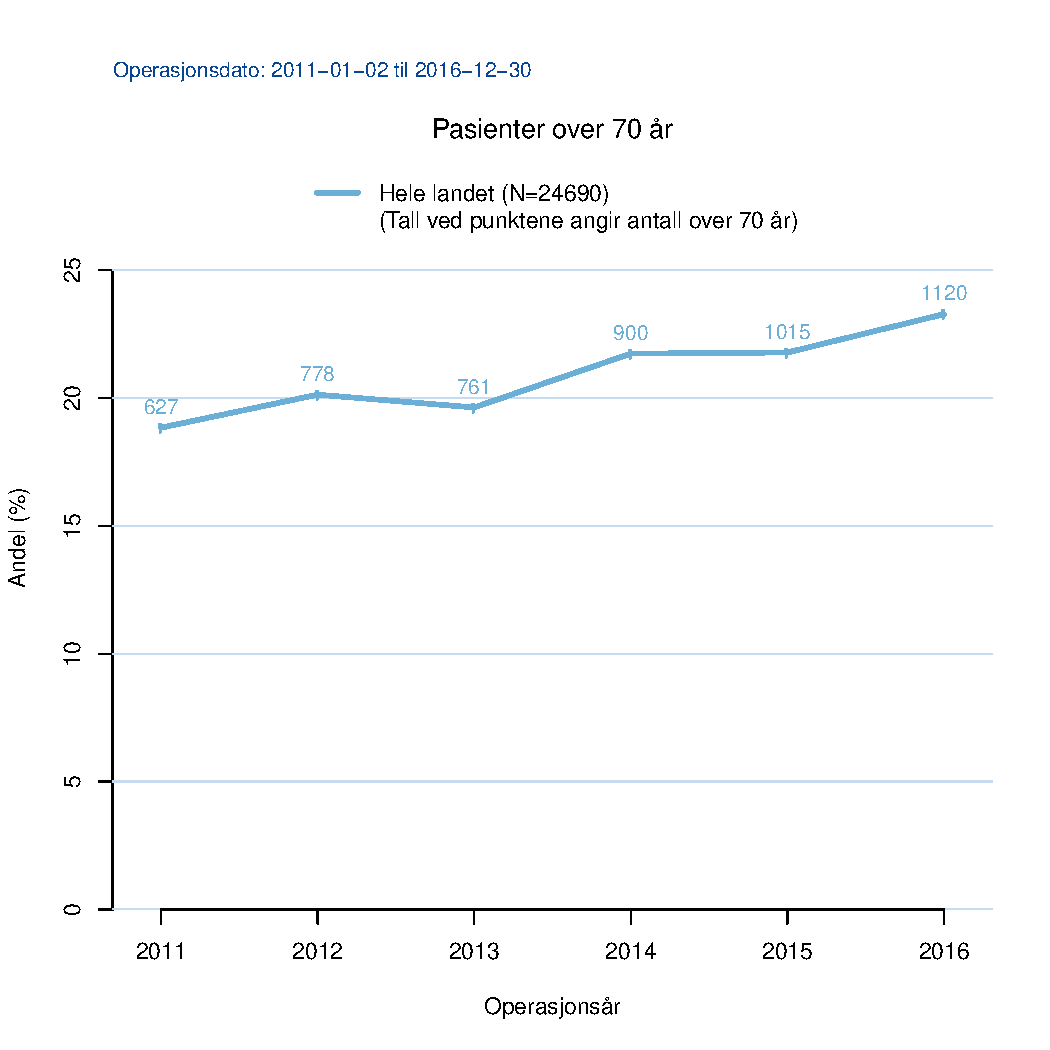
\includegraphics{Figurer/FigAlder70.pdf}}
\caption{\label{fig:Alder70} Andel ryggoperasjoner utført på personer som er 70 år eller mer.}
\end{figure}



%Figur \ref{fig:Alder} viser aldersfordeling for alle pasienter i rappAar.

%\begin{figure}[ht]
%	\centering 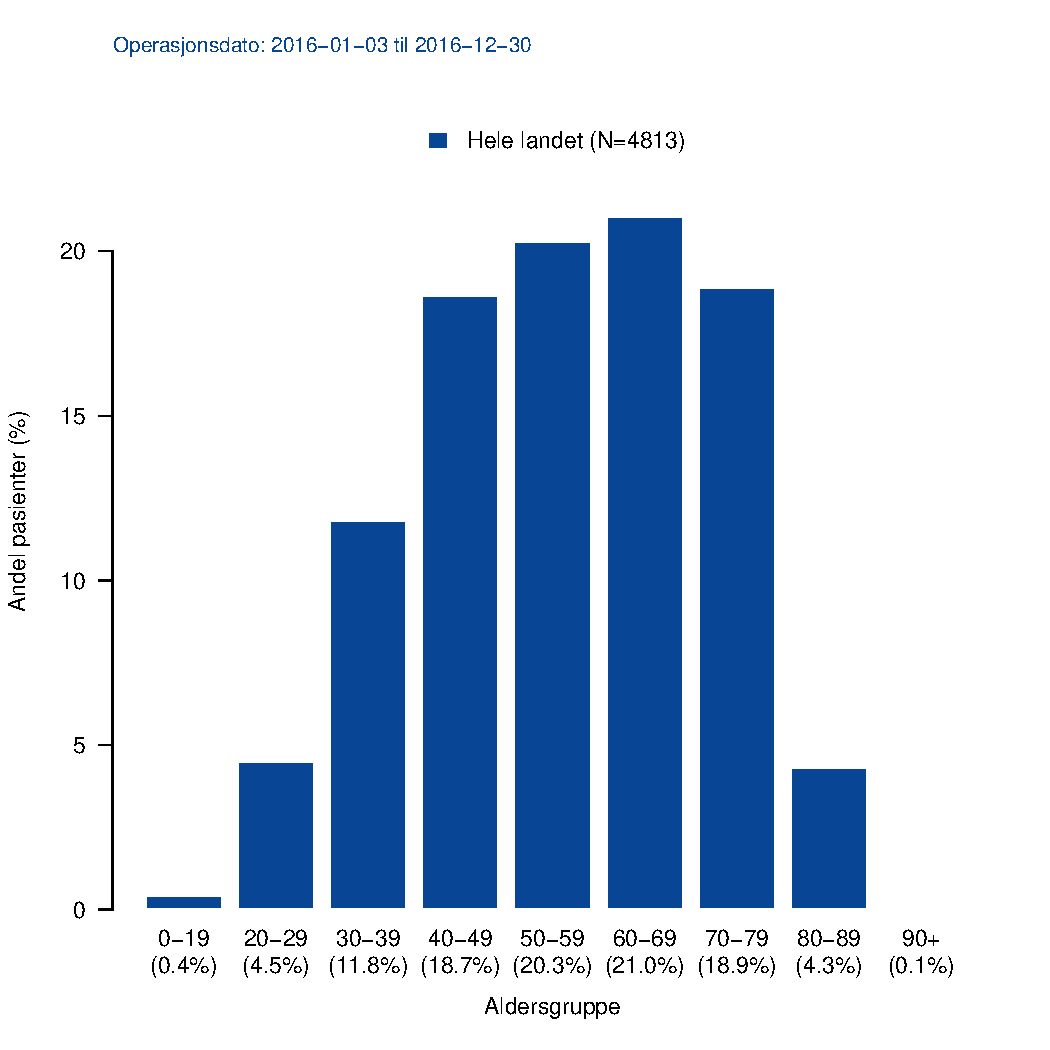
\includegraphics[width= s1\textwidth]{FigAlderFord.pdf}
%	\caption{\label{fig:Alder} paste0(AlderFord$Tittel,', ',rappAar)}
%\end{figure}

\subsection{Kroppsmasseindex (Body Mass Index, BMI)}



Opplysninger om høyde og vekt er rapportert fra pasientene selv.
Andelen pasienter med fedme har vært jevt økende fra 
20.6 \% 
i 2011
til 25.6 \%
i  2017.

Publikasjoner fra NKR viser at pasienter med fedme kan forvente signifikant mindre bedring etter 
ryggkirurgi sammenliknet med de som har lavere BMI. 




\subsection{Morsmål / etnisitet og utdanning}



Andelen fremmedspråklige (inkl. samisk) som opereres har økt fra 4.6 \% til 6.9 \% i perioden 2011 til 2017.\\
Beslutning om ryggkirurgi baserer seg på en felles forståelse mellom kirurg og
pasient av hva helseproblemene består i og hva som kan oppnås med operasjon
(«shared desicion making»). I behandling av fremmedspråklige er kommunikasjon
en utfordring. Eksempelvis var suksessraten ved lumbal prolapskirurgi for de med norsk som morsmål 65 \% mot 56 \% 
\textit{Tore sjekk tall} 
for fremmedspråklige. Bedre kommunikasjon (f.eks. ved hjelp av tolketjeneste) kan teoretisk bidra til å redusere disse
forskjellene. Figur \ref{fig:Morsmal} viser andelen fremmedspråklige operert ved de ulike avdelingene i 2017.

\begin{figure}[ht]
\scalebox{0.7}{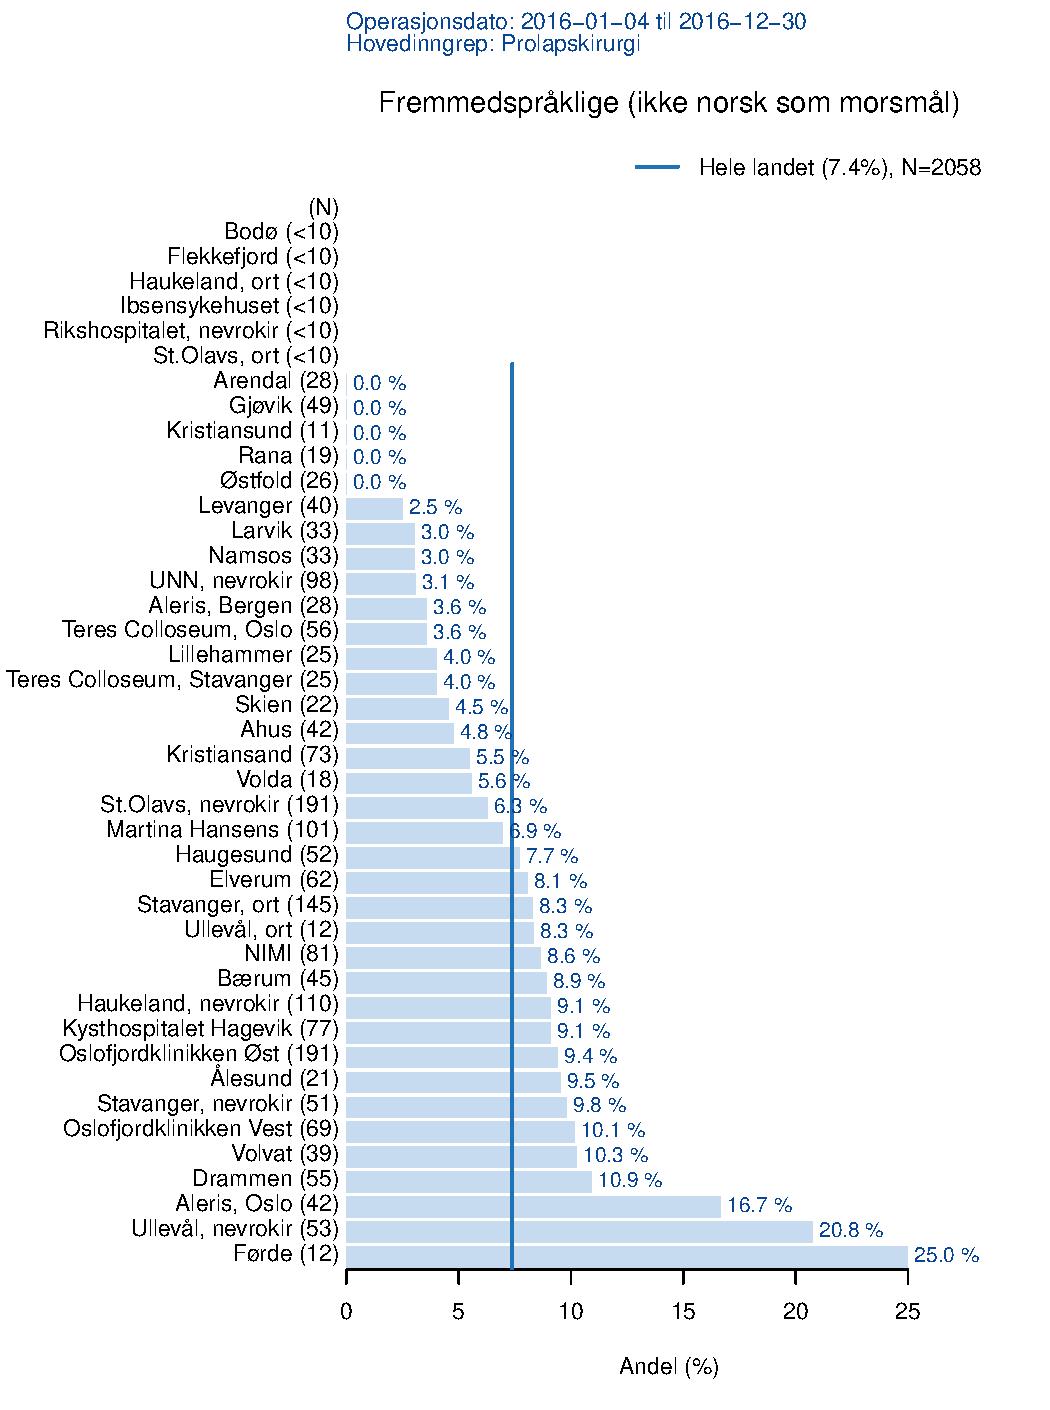
\includegraphics{Figurer/FigMorsmal.pdf}}
\caption{\label{fig:Morsmal} Andel fremmedspråklige av alle ryggopererte ved ulike sykehus i
Norge.}
\end{figure}




Lav utdanning er assosiert til dårligere operasjonsresultat. Andelen ryggopererte med høyere utdanning (høyskole eller universitet) var 36.6 i 2017 mot  30.9 i 2011. 
Opplysningene om utdanning er rapportert av pasientene selv. 
Figur \ref{fig:HoyUtdAvd} viser andel ryggopererte 
med høyskole eller universitetsutdanning ved hvert sykehus/avdeling.


\begin{figure}[ht]
\scalebox{0.7}{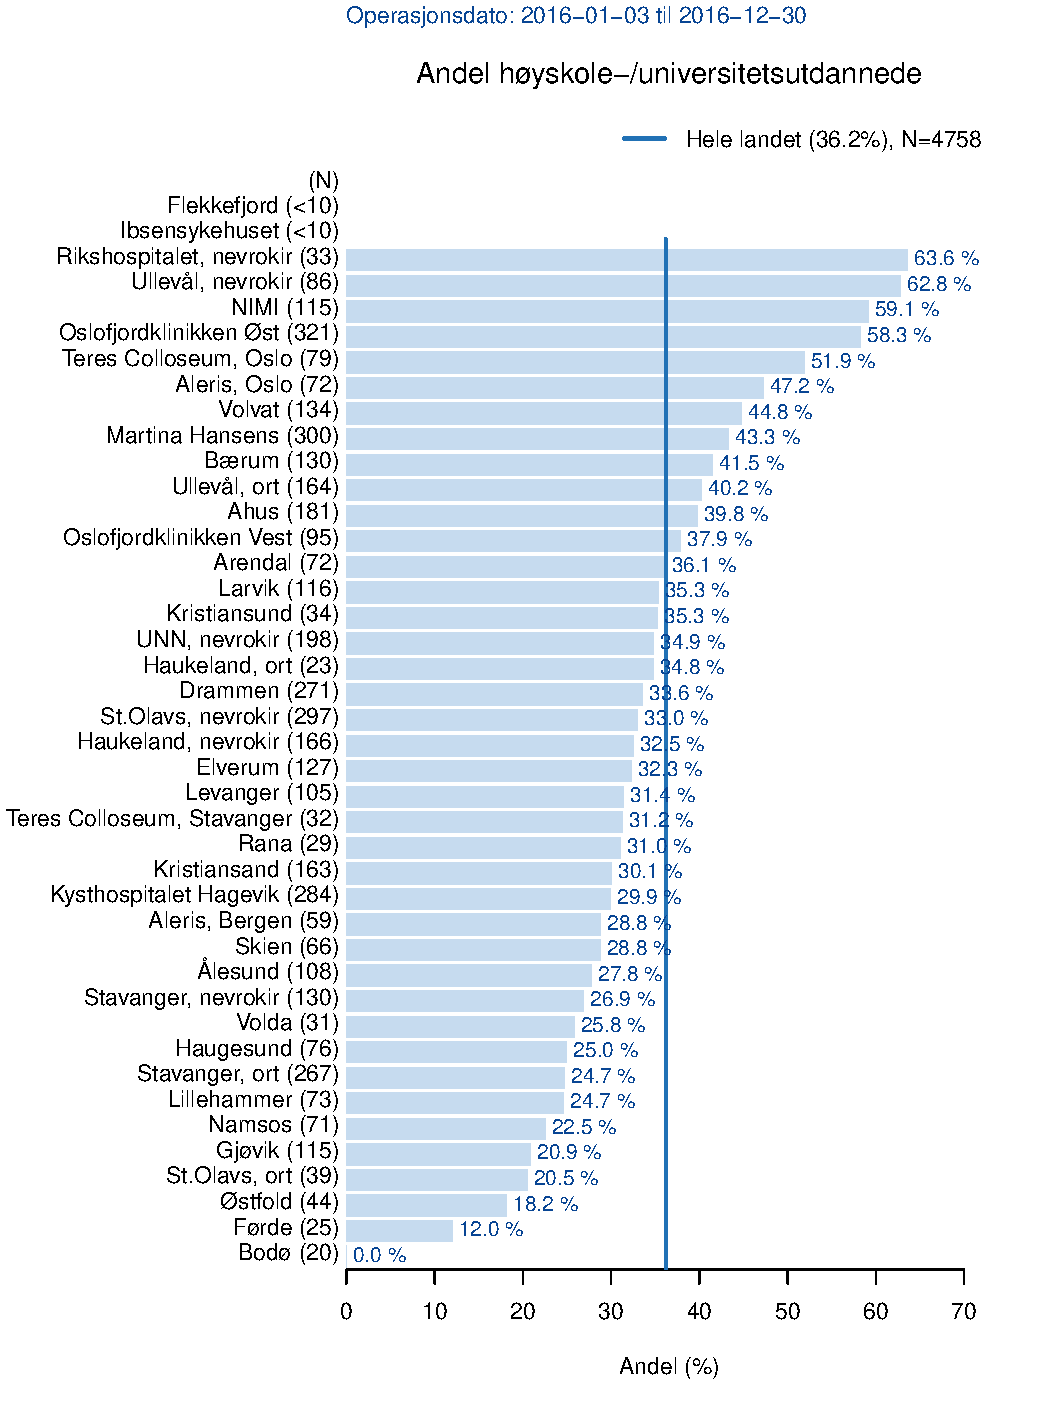
\includegraphics{Figurer/FigHoyUtdAvd.pdf}}
\caption{\label{fig:HoyUtdAvd} Andel pasienter med høyere utdanning (høyskole/universitet).}
\end{figure}


\clearpage
Avdelinger som har en pasientpopulasjon med lav utdanning og mange fremmedspråklige pasienter vil kunne forvente svakere operasjonsresultater bedømt ut fra pasient rapporterte resultatmål (PROM).
\subsection{Arbeidsstatus}
Kun  20% er i fullt arbeid når de blir ryggoperert.

% latex table generated in R 3.5.0 by xtable 1.8-2 package
% Mon Oct 01 09:27:14 2018
\begin{table}[ht]
\centering
\begin{tabular}{lr}
  \hline
 & Andeler \\ 
  \hline
I arbeid & 19.8\% \\ 
  Hjemmeværende & 1.3\% \\ 
  Student/skoleelev & 1.3\% \\ 
  Pensjonist & 31.1\% \\ 
  Arbeidsledig & 1.5\% \\ 
  Sykemeldt & 20.6\% \\ 
  Aktiv sykemeldt & 0.9\% \\ 
  Delvis Sykemeldt & 7\% \\ 
  Attføring/rehabiliteirng & 4.2\% \\ 
  Uføretrygdet & 12.3\% \\ 
   \hline
\end{tabular}
\caption{Arbeidsstatus, pasienter operert i 2017.} 
\label{tab:Arb}
\end{table}


Tabell \ref{tab:Arb} viser fordeling av arbeidsstatus før operasjon for de 98.5\% 
av pasientene i registeret som har svart på spørsmål om arbeidsstatus. 
Andelen pasienter som mottok sykepenger (sykemeldte, uføretrygdede eller personer 
på attføring) og av den grunn var helt eller delvis ute av jobb før operasjonen var 
45 \%. 

%\clearpage


\subsection{Uføretrygd og erstatning }




Pasienter som har en uavklart uføre eller erstatningssak vil sjeldnere komme tidlig tilbake i jobb etter operasjon og rapporterer mindre helseforbedringer etter operasjon. Sykehus som opererer en høy andel av denne pasientkategorien vil følgelig få dårligere resultater bedømt ut fra PROM og arbeidstilknytning.
Både andel som har søkt eller planlegger å søke uføretrygd eller erstatning ligger stabilt og var i 2017 
henholdsvis 4.7 \% og 4.5 \%. 
Figur \ref{fig:Ufor} viser andel ryggopererte ved hver avdeling som har søkt eller planlegger å søke uføretrygd.

\begin{figure}[ht]
\scalebox{0.7}{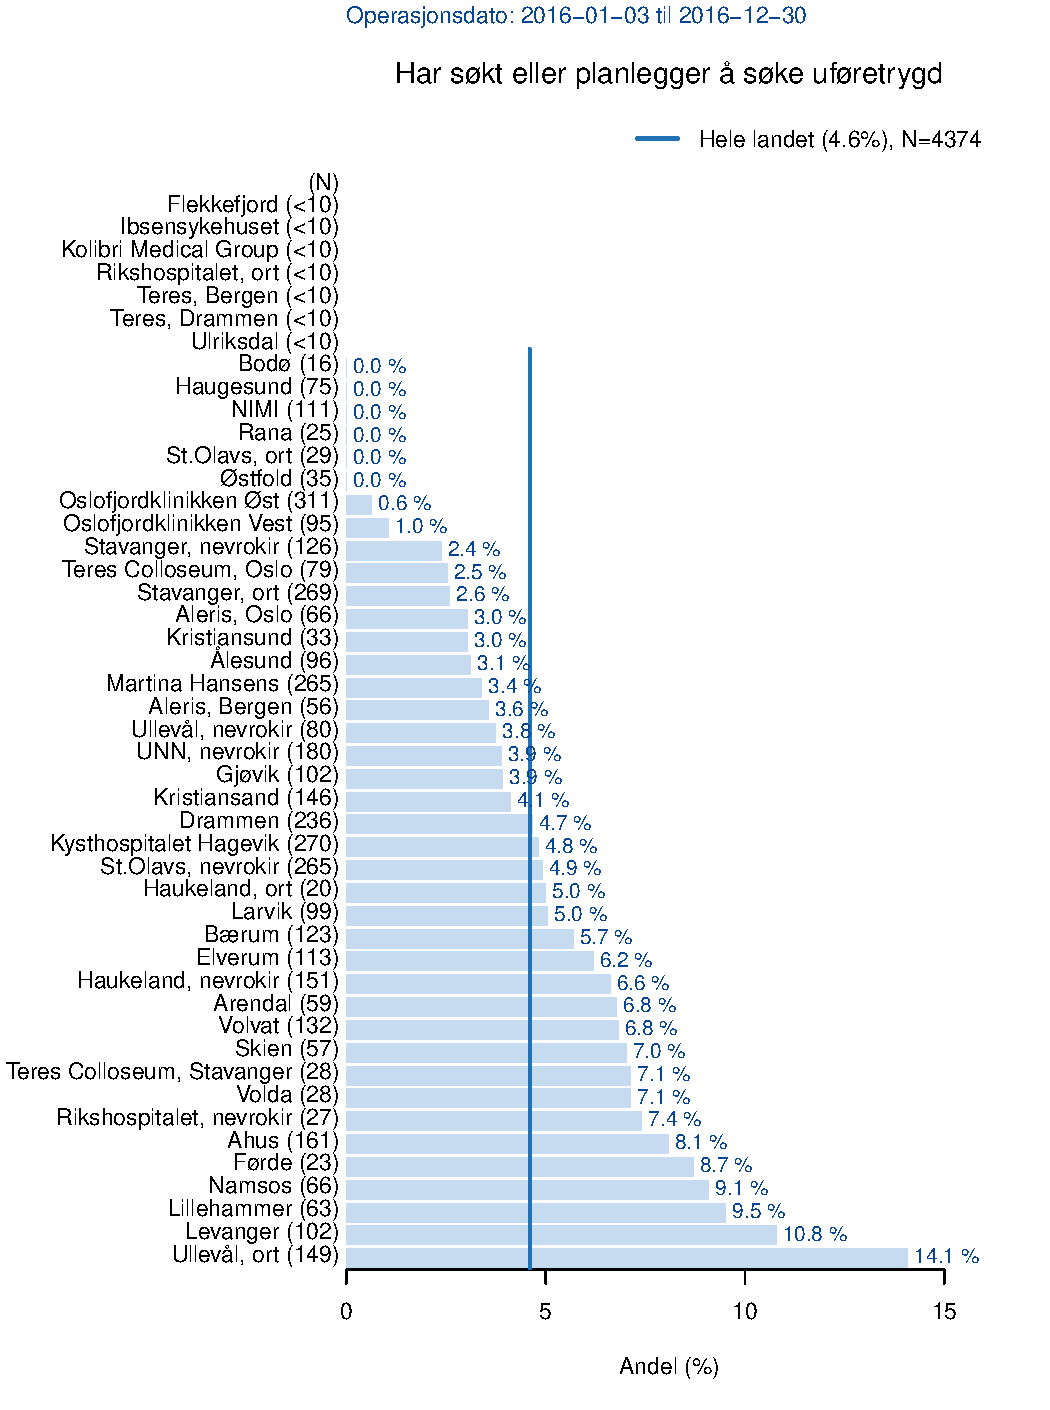
\includegraphics{Figurer/FigUforAvd.pdf}}
\caption{\label{fig:Ufor} Andel pasienter som har søkt eller planlegger å søke uføretrygd i 2017} 
\end{figure}


\clearpage

\subsection{Tidligere ryggoperert}
Informasjonen er hentet fra legeskjema.
%Figur \ref{fig:TidlOp} viser en prosentvis fordelig mellom primæroperasjon, det vil si første gangs 
%operasjon, og operasjoner hos pasienter som har vært operert tidligere.  
%Søylene representerer hvert år frem til i dag. Tallet på toppen av søylen viser antall operasjoner utført 
%det aktuelle året. 
Reoperasjoner har generelt dårligere effekt enn første gangs operasjon.





Andelen reoperasjoner var 25 \% i 2011 og 27 \% i 2017.
Av de pasientene operert i 2017 som hadde vært operert tidligere, var 57.6\% 
operert i samme nivå, 33.7\% 
operert i annet nivå og 8.6\% 
operert i både samme og annet nivå.




NKR har tidligere vist at multiple reoperasjoner har minimal effekt. Andelen som har vært operert 
mer enn 2 ganger tidligere ligger mellom 0.9 \%
og 1.6 \% for prolapspasienter og mellom 1.7 \%
og 3.1 \% for lumbal spinal stenosepasienter i perioden 2011-2017. 
Det gjenstår å evaluere om undergrupper av pasientene kan ha god nytte av flere reoperasjoner og type kirurgi som kan være mest aktuell for dem.


\subsection{ASA-grad og røyking}
ASA angir pasientens fysiske ”sårbarhet” ved anestesi og operasjon på en skala fra 1 til 5. 
Opplysningene hentes fra legeskjema.
% latex table generated in R 3.5.0 by xtable 1.8-2 package
% Mon Oct 01 09:27:21 2018
\begin{table}[ht]
\centering
\begin{tabular}{crr}
  \hline
 & Antall & Prosent \\ 
  \hline
I & 1362 & 25.8\% \\ 
  II & 3090 & 58.6\% \\ 
  III & 784 & 14.9\% \\ 
  IV & 10 & 0.2\% \\ 
  V & 1 & 0\% \\ 
  Ikke besvart & 25 & 0.5\% \\ 
   \hline
\end{tabular}
\caption{Fordeling av ASA-grad, operasjoner utført i 2017} 
\label{tab:ASA}
\end{table}


Tabell \ref{tab:ASA} viser fordeling av ASA grad. Andelen pasienter med ASA grad I-II 
var 84.4\%. Pasienter som røyker, havner 
automatisk i ASA-grad II eller høyere. Data fra NKR har vist at røyking er assosiert til dåligere operasjonsresultat.
Mange kirurger krever eller anbefaler røykeslutt før mer omfattende inngrep slik som fusjonskirurgi.
%txt
Andel røykere som ryggopereres har gått ned fra 28.2 \% i 2011 til 19.1 \% i 2017. 



\subsection{Radiologisk utredning}

Tabell \ref{tab:RV} viser hvor stor andel av pasientene som har vært til ulike typer 
radiologisk undersøkelser. En pasient kan ha vært til flere undersøkelser. Hyppigste radilologiske diagnoser er skiveprolaps og spinal stenose.
Spørsmålene er besvart av leger. 

% latex table generated in R 3.5.0 by xtable 1.8-2 package
% Mon Oct 01 09:27:23 2018
\begin{table}[ht]
\centering
\begin{tabular}{lrr}
  \hline
 & Antall & Andeler \\ 
  \hline
CT & 371 & 7\% \\ 
  MR & 5175 & 98\% \\ 
  Radikulografi & 38 & 1\% \\ 
  Diskografi & 2 & 0\% \\ 
  Diagnostisk blokade & 28 & 1\% \\ 
  Røntgen LS-columna & 1208 & 23\% \\ 
  Med fleksjon/ekstensjon & 394 & 7\% \\ 
  Tot. ant. & 5272 &   \\ 
   \hline
\end{tabular}
\caption{Radiologisk vurdering, 2017} 
\label{tab:RV}
\end{table}




Tabell \ref{tab:RF} viser diagnoser basert på radiologiske funn hos alle pasienter 
i 2017. 
Spørsmålene er besvart av leger.
En pasient kan ha flere diagnoser.
%txtRFnorm


% latex table generated in R 3.5.0 by xtable 1.8-2 package
% Mon Oct 01 09:27:23 2018
\begin{table}[ht]
\centering
\begin{tabular}{lrr}
  \hline
 & Antall & Andeler \\ 
  \hline
Skiveprolaps & 2346 & 44\% \\ 
  Sentral spinalstenose & 1755 & 33\% \\ 
  Lateral spinalstenose & 1771 & 34\% \\ 
  Foraminal stenose & 636 & 12\% \\ 
  Degenerativ rygg/skivedegenerasjon & 926 & 18\% \\ 
  Istmisk spondylolistese & 143 & 3\% \\ 
  Degenerativ spondylolistese & 521 & 10\% \\ 
  Degenerativ skoliose & 155 & 3\% \\ 
  Synovial syste & 144 & 3\% \\ 
  Pseudomeningocele & 1 & 0\% \\ 
  Tot.ant. & 5272 &   \\ 
   \hline
\end{tabular}
\caption{Radiologiske diagnoser, 2017} 
\label{tab:RF}
\end{table}





\section{Virksomhetsdata}

Andelen som er operert ved hjelp av synsfremmende midler (mikroskop eller
lupebriller), som har åpenbare fordeler, har økt fra 86 \% i 2011 til 
98 \% i 2017 for lumbalt prolaps. 
Tilsvarende tall for lumbal spinal stenose var en økning fra 68 \% i 2011 til 
98 \% i 2017.



\subsection{Type operasjon}



De hyppigste tilstandene pasienter ble operert for i 2017 var lumbalt prolaps (41 \%) og spinal stenose (42 \%). Tabell \ref{tab:AntHovedInngrep} viser fordeling av hovedinngrepstype, samt antall registrerte operasjoner for hver hovedinngrepstype.
''Foramenotomi'' betyr at det er gjort dekompresjon for lumbal spinal stenose med bevaring av midtlinjestrukturer. 

% latex table generated in R 3.5.0 by xtable 1.8-2 package
% Mon Oct 01 09:27:24 2018
\begin{table}[ht]
\centering
\begin{tabular}{lrr}
  \hline
 & Antall & Andeler \\ 
  \hline
Udefinerbart & 161 & 3\% \\ 
  Prolapskirurgi & 2161 & 41\% \\ 
  Foramenotomi & 2087 & 40\% \\ 
  Laminektomi & 191 & 4\% \\ 
  Interspin. implantat & 1 & 0\% \\ 
  Fusjonskirurgi & 598 & 11\% \\ 
  Skiveprotese & 45 & 1\% \\ 
  Rev. av implantat & 28 & 1\% \\ 
   \hline
\end{tabular}
\caption{Fordeling av hovedinngrep, 2017} 
\label{tab:AntHovedInngrep}
\end{table}



%\begin{figure}[ht]
%      \scalebox{s1}{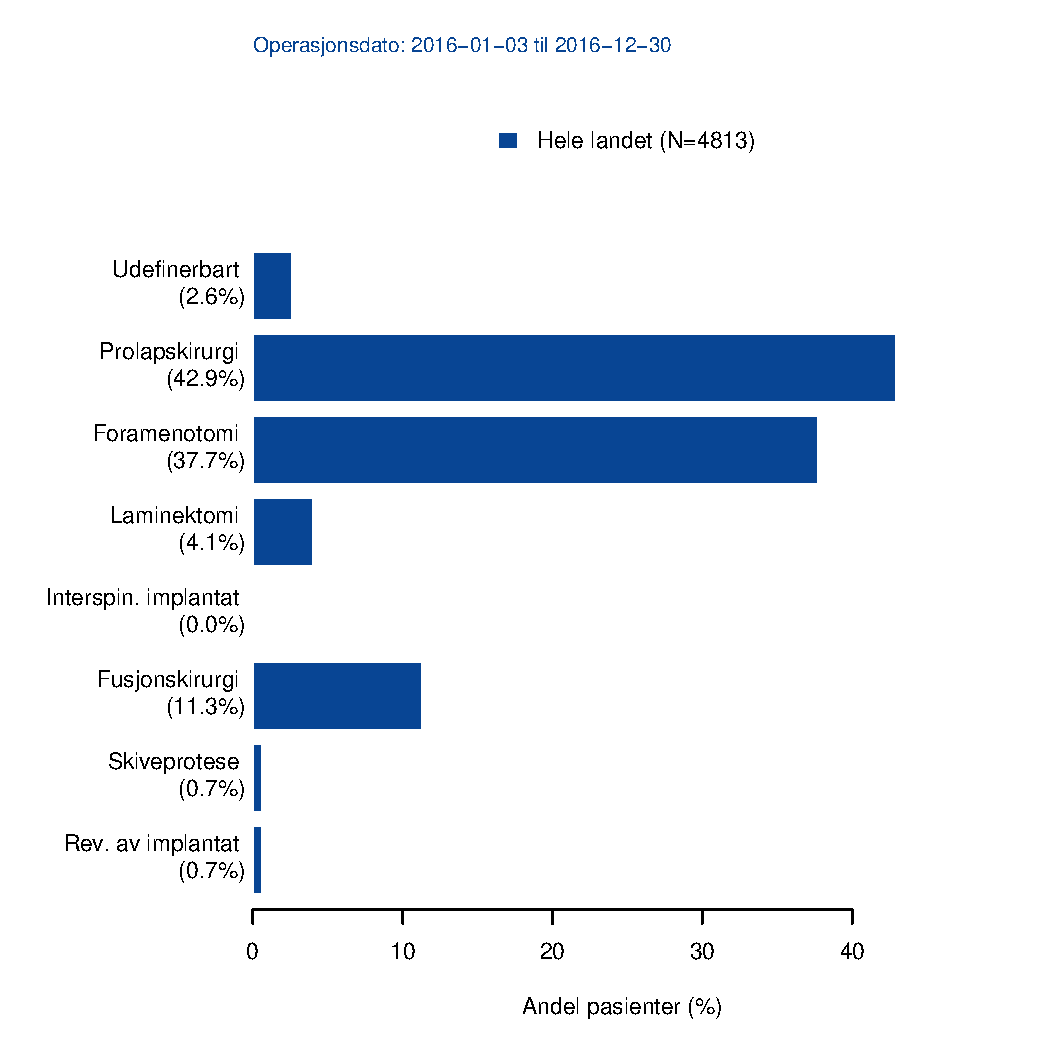
\includegraphics{Figurer/HovedInngrep.pdf}}
%      \caption{\label{fig:HovedInngrep} HovedInngrep$Tittel}
%\end{figure}



\subsubsection{Degen. spondylolistese operert med fusjonskirurgi}


I 2017 hadde 18.3 \% av de som ble operert for spinal stenose  også en forskyvning mellom ryggvirvlene (Degenerativ spondylolistese). I internasjonal litteratur er det sprikende anbefalinger i forhold til om de bør få tilleggsbehandling med avstivningsoperasjon (fusjonskirurgi).
 

Norske studier basert på data fra NKR har vist at tilleggseffekten er liten og assosiert til høyere kostnader (flere liggedøgn på sykehus). 
I 2018 blir det publisert en ny studie fra NKR i samarbeid med  tilsvarende registre i Sverige og Danmark. Denne viser stor forskjell i bruk av fusjonskirurgi mellom landene og at denne tilleggbehandlingen ikke er assosiert til større behandlingseffektivitet, men økte kostnader. En pågående nasjonal RCT multisenter studie skal i samarbeid med NKR evaluere om undergrupper av pasientene med spinal stenose og degenerativ spondylolistese kan ha spesiell nytte av fusjonskirurgi.
\clearpage

Figur \ref{fig:degSponFusj} viser at det er stor variasjon i bruk av fusjonskirurgi, 
for denne pasientgruppen i tidsperioden, også mellom avdelinger på samme sykehus. Nevrokirurgiske avdelinger gjør mindre fusjonskirurgi enn de ortopediske.
\begin{figure}[ht]
\scalebox{0.7}{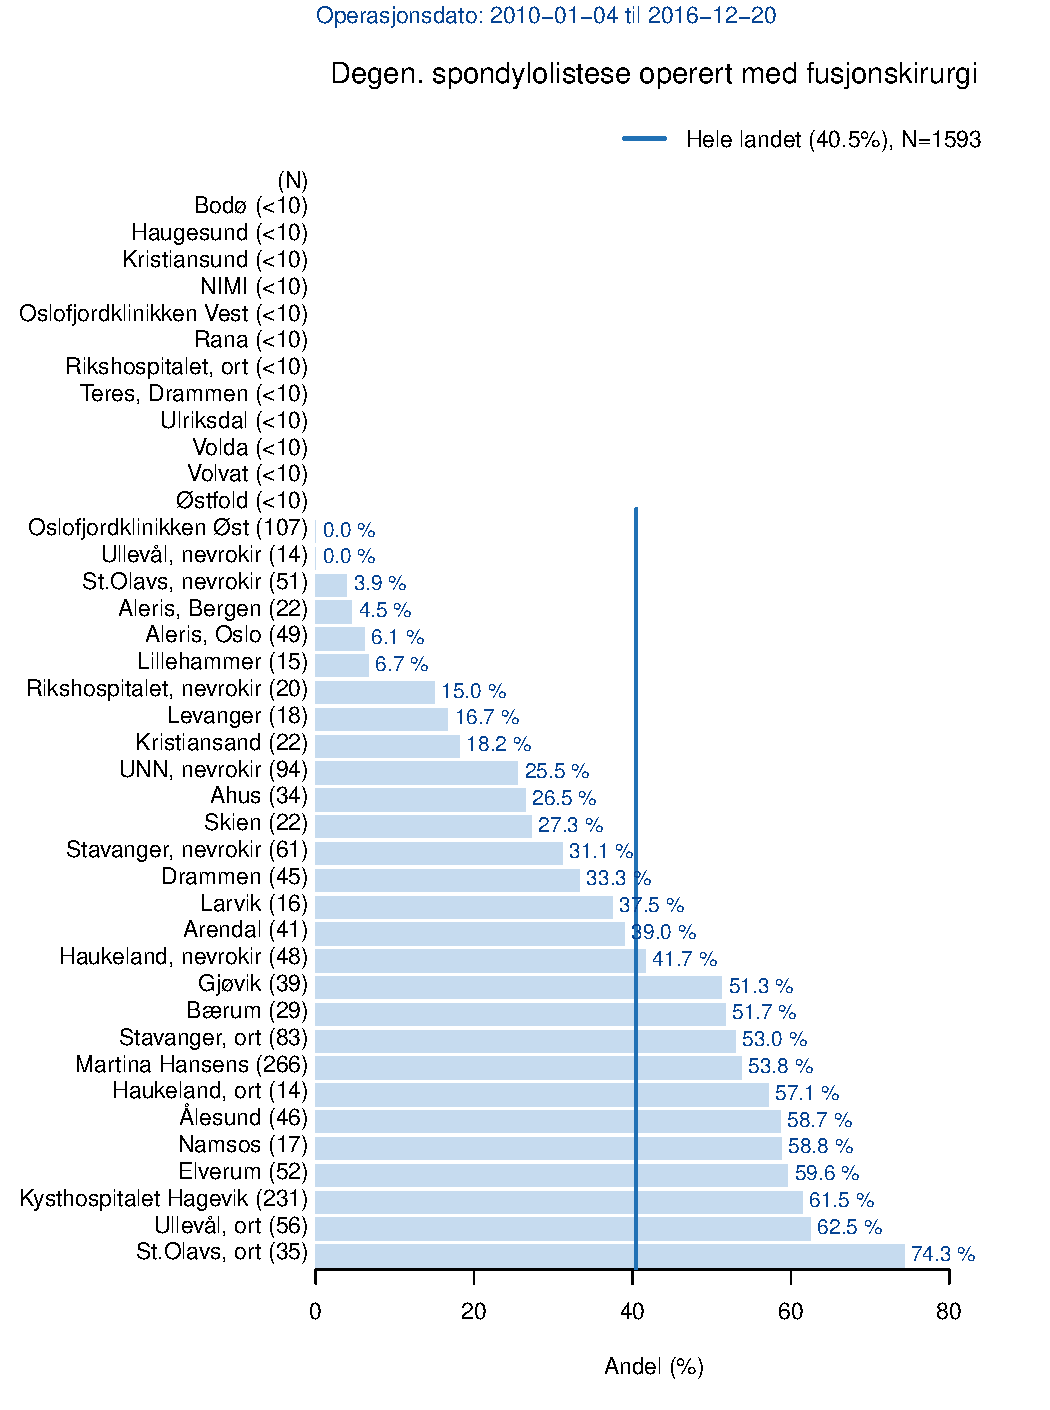
\includegraphics{Figurer/FigdegSponFusj.pdf}}
\caption{\label{fig:degSponFusj} Lumbal spinal stenose og degenerativ spondylolistese operert med fusjonskirurgi}
\end{figure}

Figur \ref{fig:degSponFusjSStid} viser at andelen som får 
tilleggsbehandling med fusjonskirurgi er redusert fra 50.9 \% 
i 2011 til 29.7 \% i 2017.

\begin{figure}[ht]
\scalebox{0.7}{\includegraphics{Figurer/FigdegSponFusjSStid.pdf}}
\caption{\label{fig:degSponFusjSStid} Andel pasienter med degenerativ spondylolistese og spinal stenose som blir operert med fusjonskirurgi per år.}
\end{figure}



\clearpage


\subsection{Liggetid}

Informasjonen er hentet fra legeskjema.
%Figur \ref{fig:Liggedogn} viser liggedøgnsfordeling for alle pasienter operert i rappAar. 
%Figur \ref{fig:LiggedognTid} viser gjennomsnittlig antall liggedøgn per år.  
Det har vært en reduksjon i liggetid  på sykehus (ca 1 døgn) fram til 2017 for både lumbal prolaps og spinal stenose opererte. 
Dette kan henge sammen med økt bruk av mindre invasive operasjonsmetoder og mer dagkirurgi. 
Andelen operert med dagkirurgi for hhv lumbalt skiveprolaps og spinal stenose har gått opp fra 
23 \% og 9 \%  i 2011 til 31 \% og 13 \%  i 2017  
Figur \ref{fig:LiggetidAvdPro} og \ref{fig:LiggetidAvdSS} viser at det var stor variasjon i antall liggedøgn mellom sykehus og avdelinger i 2017.


      
      
      
      %\begin{figure}[h] 
%\scalebox{s1}{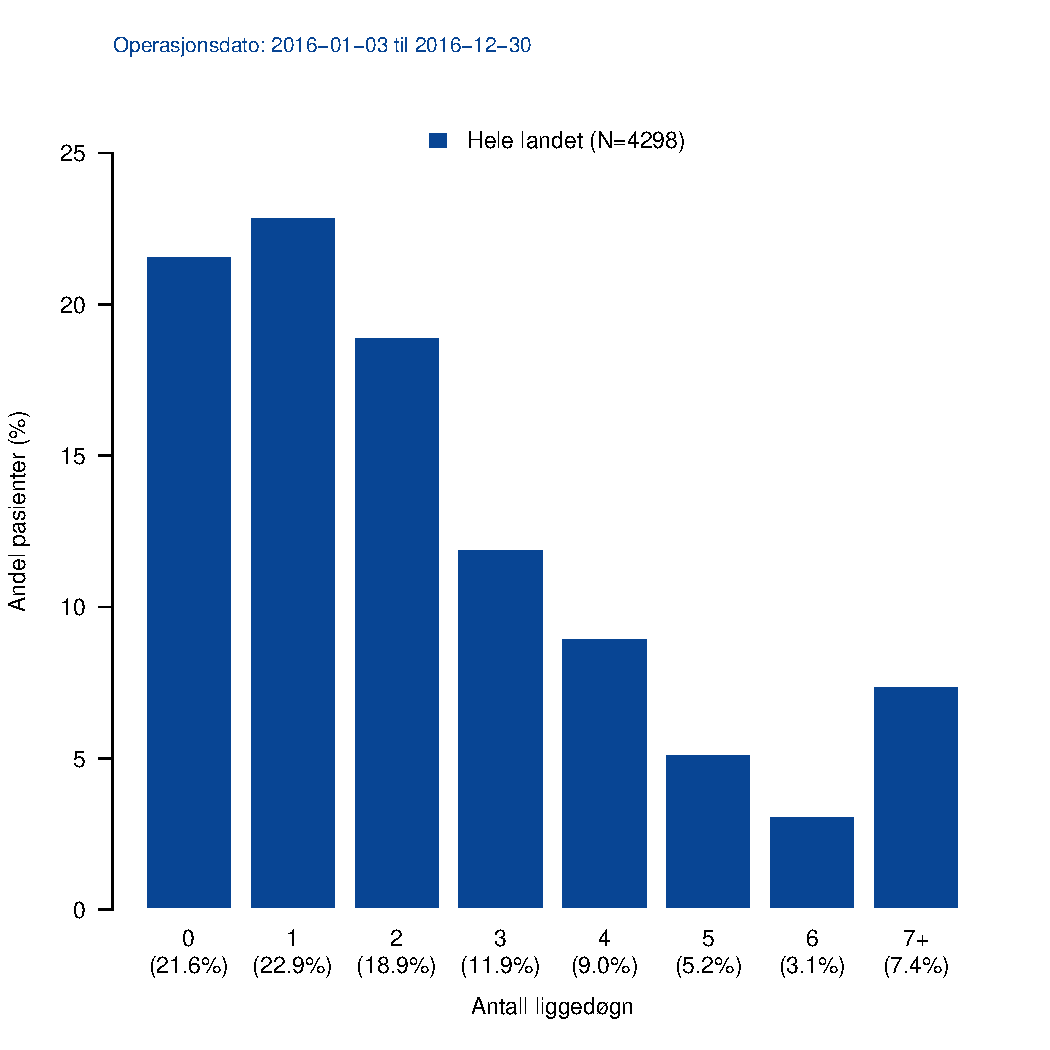
\includegraphics{Figurer/FigLiggetidFord.pdf}}
%\caption{LiggetidFord$Tittel}
%\label{fig:Liggedogn}
%\end{figure}

% \begin{figure}[h] 
% \centerline{
      % \scalebox{s2}{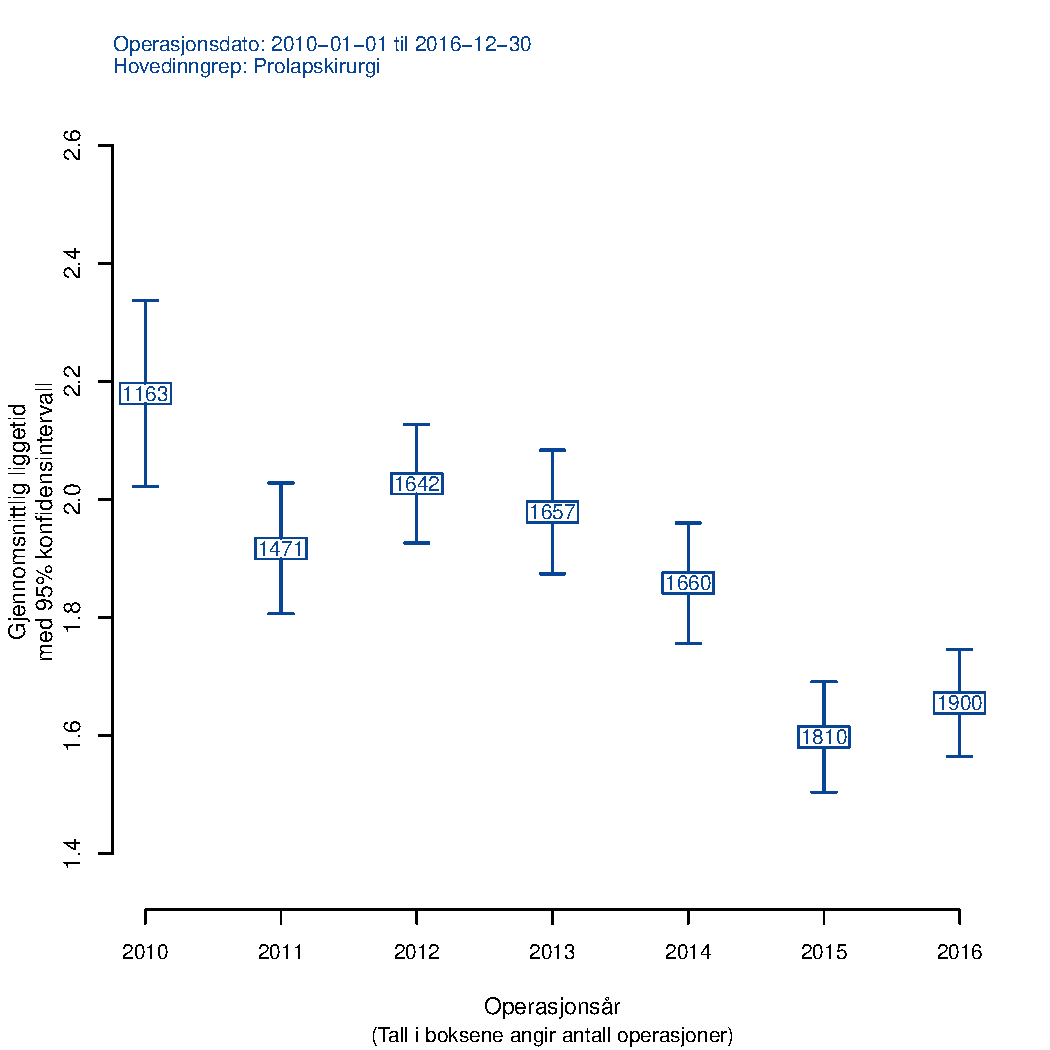
\includegraphics{Figurer/LiggetidBoxPro.pdf}}
      % \scalebox{s2}{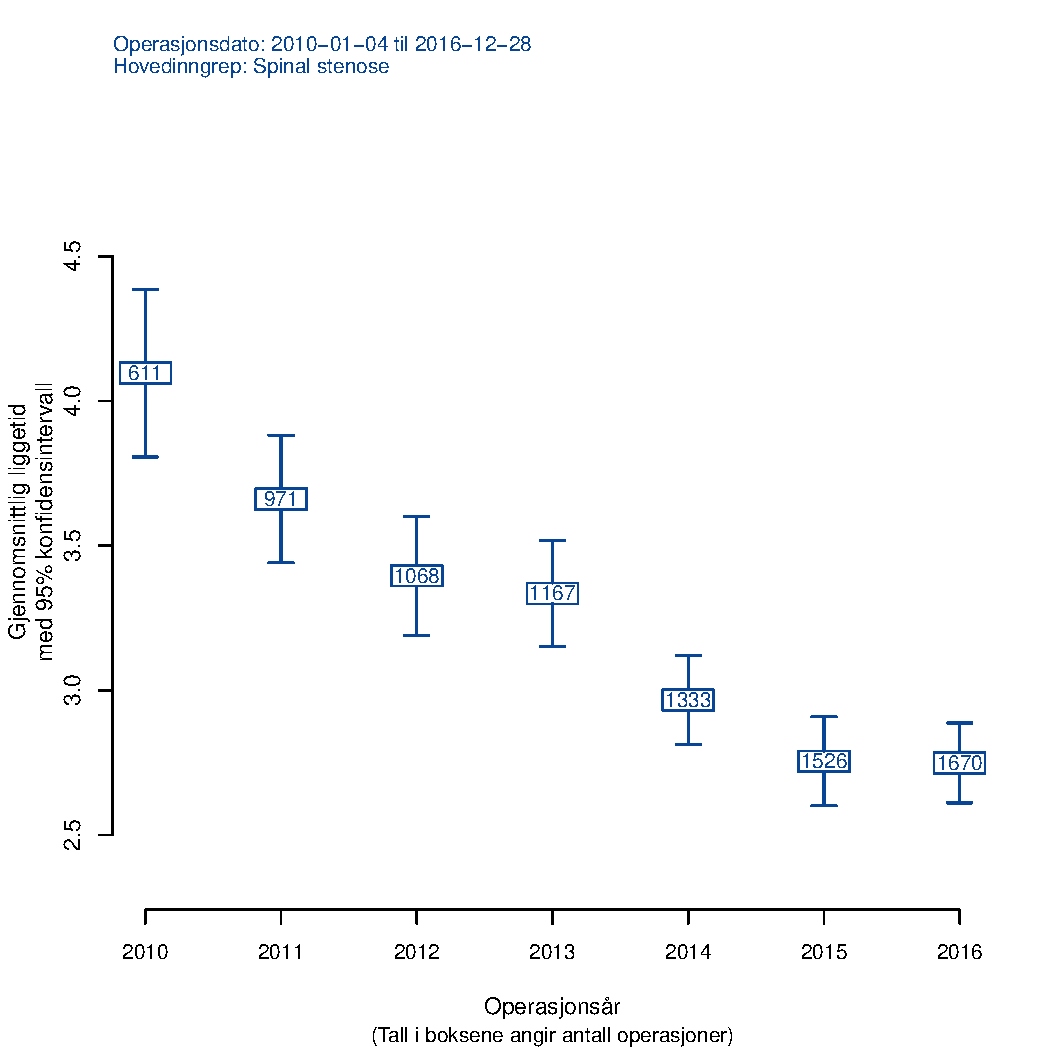
\includegraphics{Figurer/LiggetidBoxSS.pdf}}
      % }
% \caption{Gjennomsnittlig liggetid for hhv. lumbalt prolaps og spinal stenose. }
% \label{fig:LiggedognTid}
% \end{figure}

\begin{figure}[h] 
\scalebox{0.7}{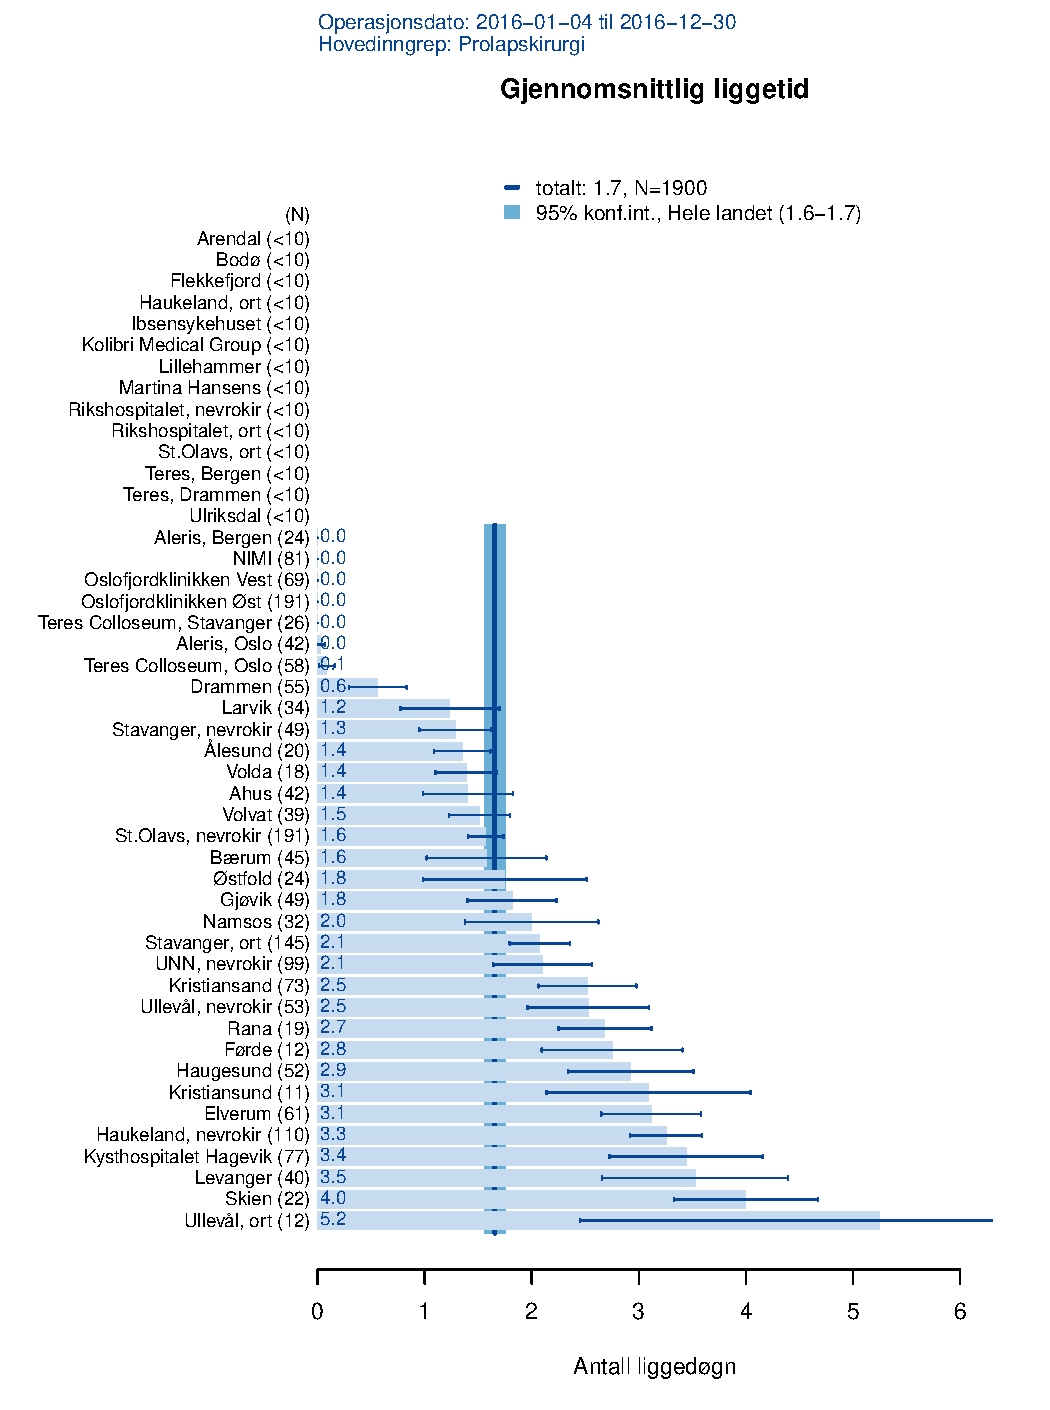
\includegraphics{Figurer/LiggetidAvdPro.pdf}}
\caption{Gjennomsnittlig liggetid for lumbalt prolaps ved ulike avdelinger i 2017. } 
\label{fig:LiggetidAvdPro}
\end{figure}

\begin{figure}[h] 
\scalebox{0.7}{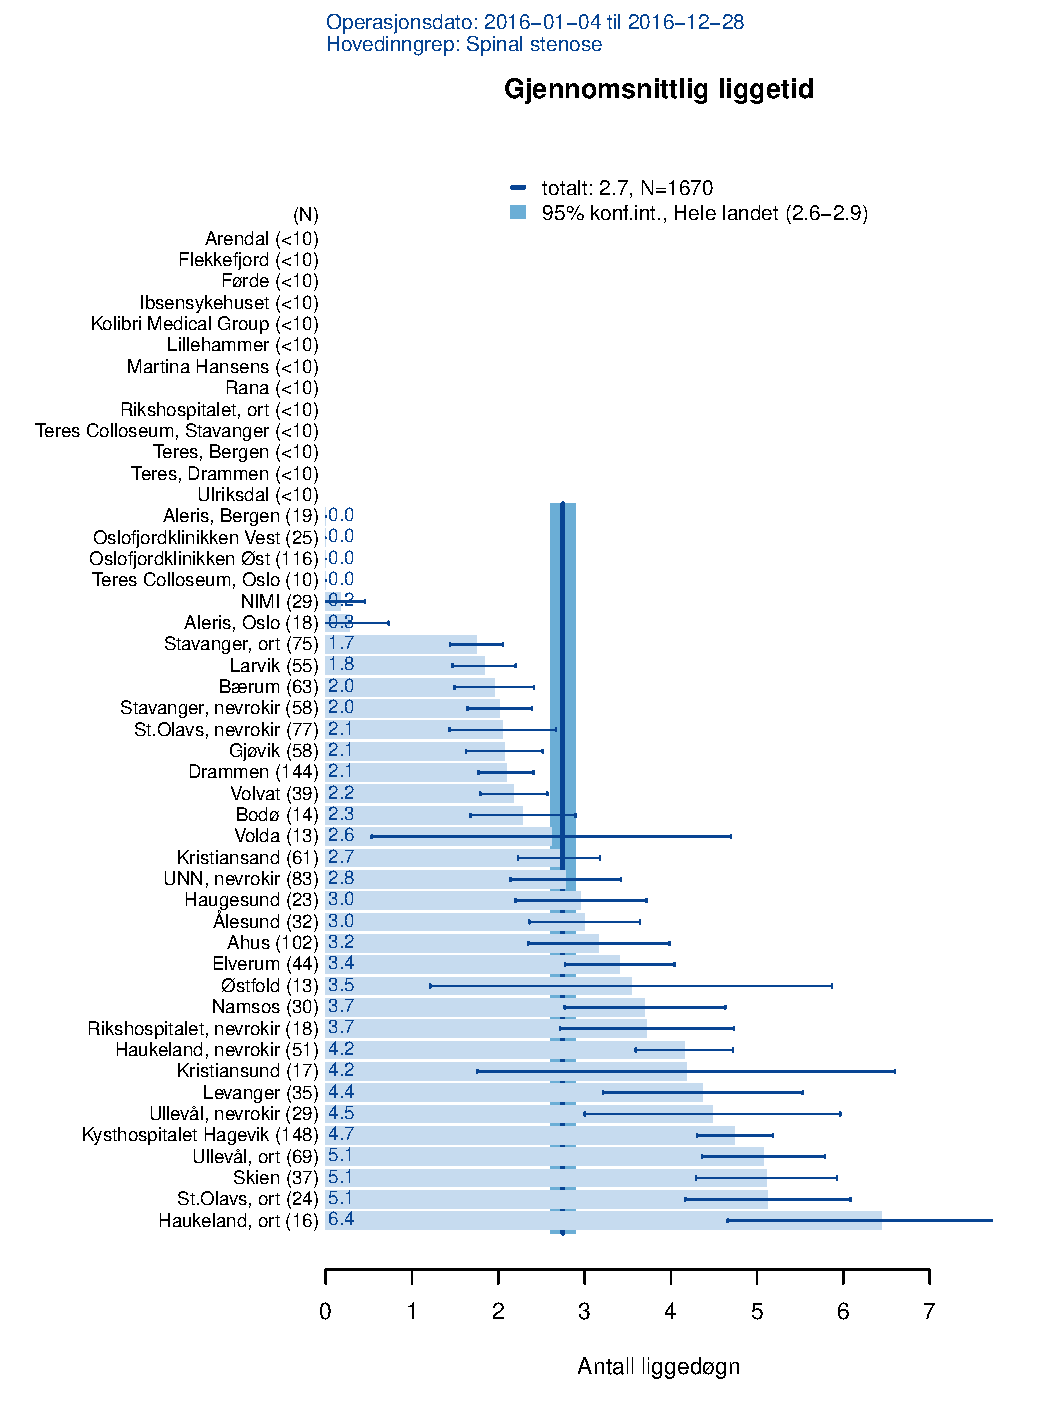
\includegraphics{Figurer/LiggetidAvdSS.pdf}}
\caption{Gjennomsnittlig liggetid for lumbal spinal stenose ved ulike avdelinger i 2017 } 
\label{fig:LiggetidAvdSS}
\end{figure}


      
      
      
      
      \clearpage

\section{Resultatmål}
All informasjon i dette kapitlet er hentet fra pasientskjema.  Viktige årsaker til variasjon i operasjonsresultat kan være at sykehusene behandler
ulike pasientgrupper med ulik risikoprofil. Ingen av resultatmålene er justert
for disse forskjellene. Noen risikofaktorer kan modifiseres/bedres gjennom bedre styring og planlegging av
virksomheten, strengere indikasjonsstilling og bedret pasientsikkerhet. Andre faktorer, for eksempel utdanningsnivå, lar seg ikke modifisere.
Sammenholdt med bakrunnsdata og virksomhetsdata kan resultatmålene imidlertid gi en pekepinn på hvor godt behandlingstilbudet fungerer på ulike sykehus. Indikasjonsstillingen («inngangsbilletten»)til kirurgi er mest avgjørende for om operasjonsresultatet blir vellykket: Fikk rett person, rett
behandling til rett tid?

Resultatmålene er utviklet gjennom forskning (valideringsstudier) i regi av NKR i samarbeid
med blant annet Nasjonalt kompetansesenter for rygg og nakke kirurgi og ulike universistessykehus i Norge. Noen få er hentet fra annen
internasjonal litteratur. De terskelverdiene som brukes er med andre ord forskningsbaserte.
 
\textbf{Det er viktig å merke seg at pasienter som er operert i 2016 først får resultater fra ettårs oppfølgning i 2017.} 


      
      


      
      \subsection{ Resultater etter ryggkirurgi, 2011 til 2017}

\subsection{Oswestry Disability Index (ODI)}


      
      
      
      ODI brukes som hovedeffektmål og uttrykker smerterelatert  fysisk funksjon i dagliglivets aktiviteter og sykdomsspesifikk livskvalitet hos ryggpasienter. Skalaen går fra 0
til 100, hvor 0 angir ingen funksjonshemming og følgelig beste livskvalitet.

I tillegg angir pasienten smerteintensitet i henholdsvis ben og rygg på en numerisk smerteskala (NRS), 
fra 0 (ingen smerte) til 10 (verst tenkelige smerte).
\\

For lumbalt prolaps kirurgi var gjennomsnittlig ODI score rapportert i 2017 46.4 før operasjon og 16.7 ett år etter. Dette betyr at funksjonssvikten ble redusert 
fra alvorlig til minimal for gjennomsnittspasienten. 
Pasienter operert for lumbal spinal stenose fikk også
betydelig bedring (ODI redusert fra 39.2 (betydelig funksjonssvikt) til 23.2) (lett til moderat funksjonssvikt) ett år etter kirurgi. 
De som ble operert med fusjonkirurgi har
omtrent samme forbedring. ODI ble redusert fra 42.0 til 25.1). Resultatene synes å være omtrent de samme fra år til år. Suksessrate, det vil si forbedring av ODI på mer enn 20 poeng, ligger stabilt rundt 60 \% for prolapspasienter, ett år etter operasjon. 
For spinal stenosepasienter ligger "suksessraten"  ett år etter operasjon (forbedring av ODI på mer enn 30 \%) stabilt rundt 60\%.
Dette betyr at selv om
pasientene kan forvente en betydelig bedring, vil mange fortsatt ha en del restplager
ett år etter kirurgi. \\
 
 NKR
sammenstiller også norske resultater tilsvarende registre i Sverige og
Danmark. Indikasjonsstillen for kirurgi er lik og resultatene synes å være de samme i de tre nordiske landene.
Resultatene varierer imidlertid mye mellom sykehus og fra pasient til pasient. \\

%Figur \ref{fig:OswEndr} viser gjennomsnittlig endring av ODI fra før operasjon til ett år etter.





      
      Figurene \ref{fig:OswEndrAvdPro} og \ref{fig:OswEndrAvdSS} viser gjennomsnittlig endring 12 måneder etter for hver avdeling for henholdsvis prolaps og spinal stenose pasienter. Forskjellene er små. Vi ser også at konfidensintervallene er relativt brede og overlappende.

\begin{figure}[h] 
\scalebox{0.7}{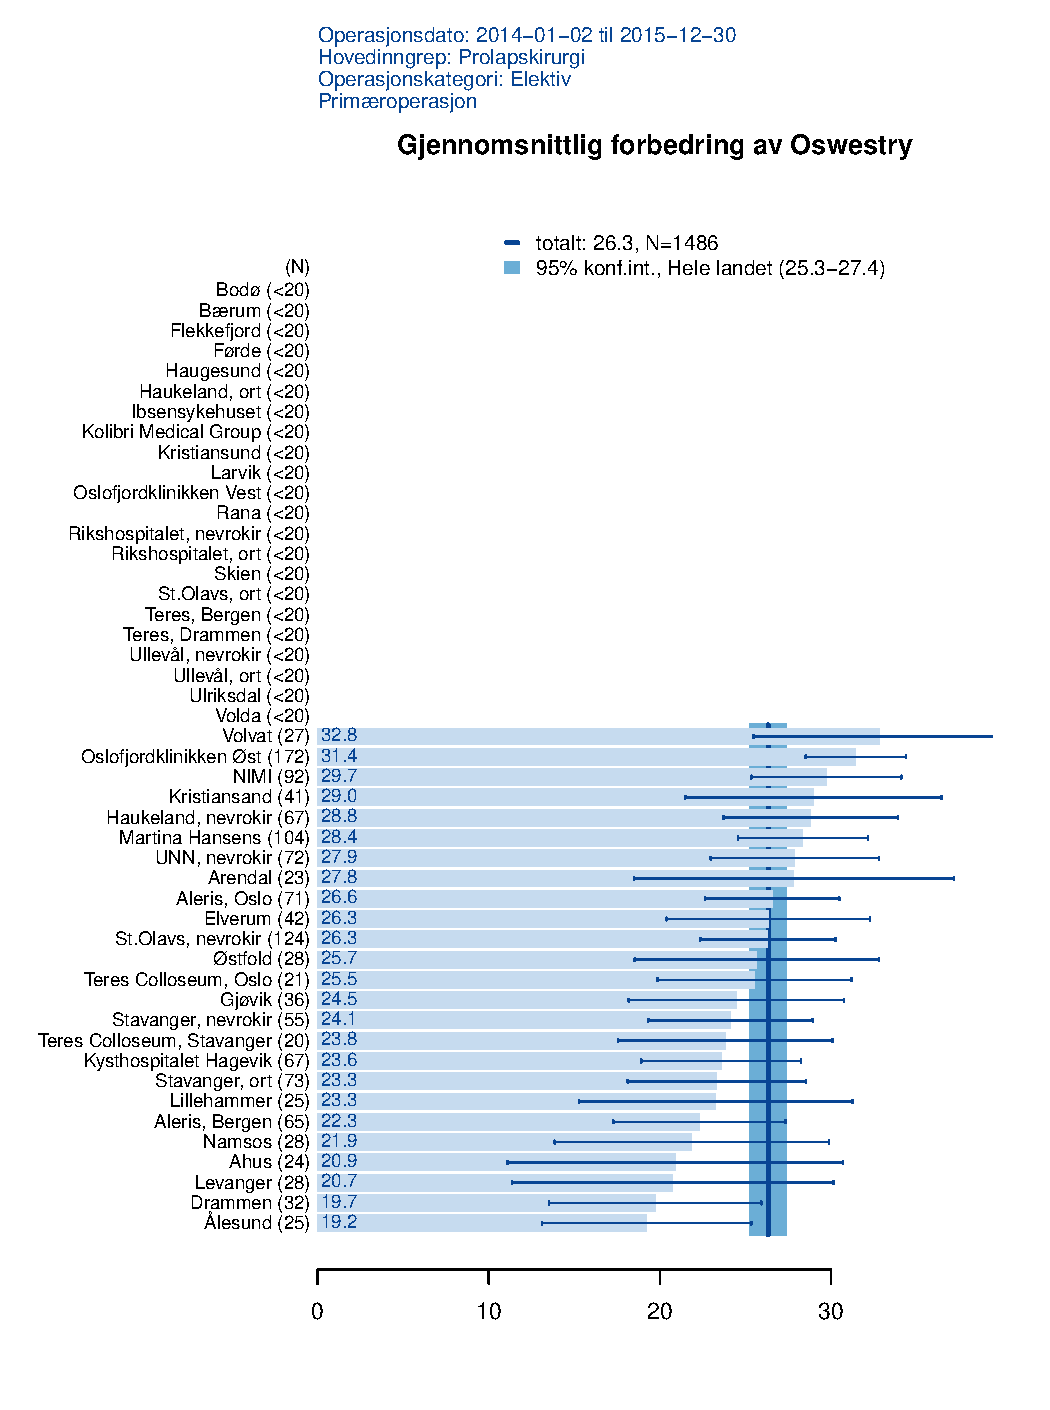
\includegraphics{Figurer/OswEndrAvdPro.pdf}}
\caption{Gjennomsnittlig endring av ODI per avdeling for lumbalt prolaps.}
\label{fig:OswEndrAvdPro}
\end{figure}

\begin{figure}[h] 
\scalebox{0.7}{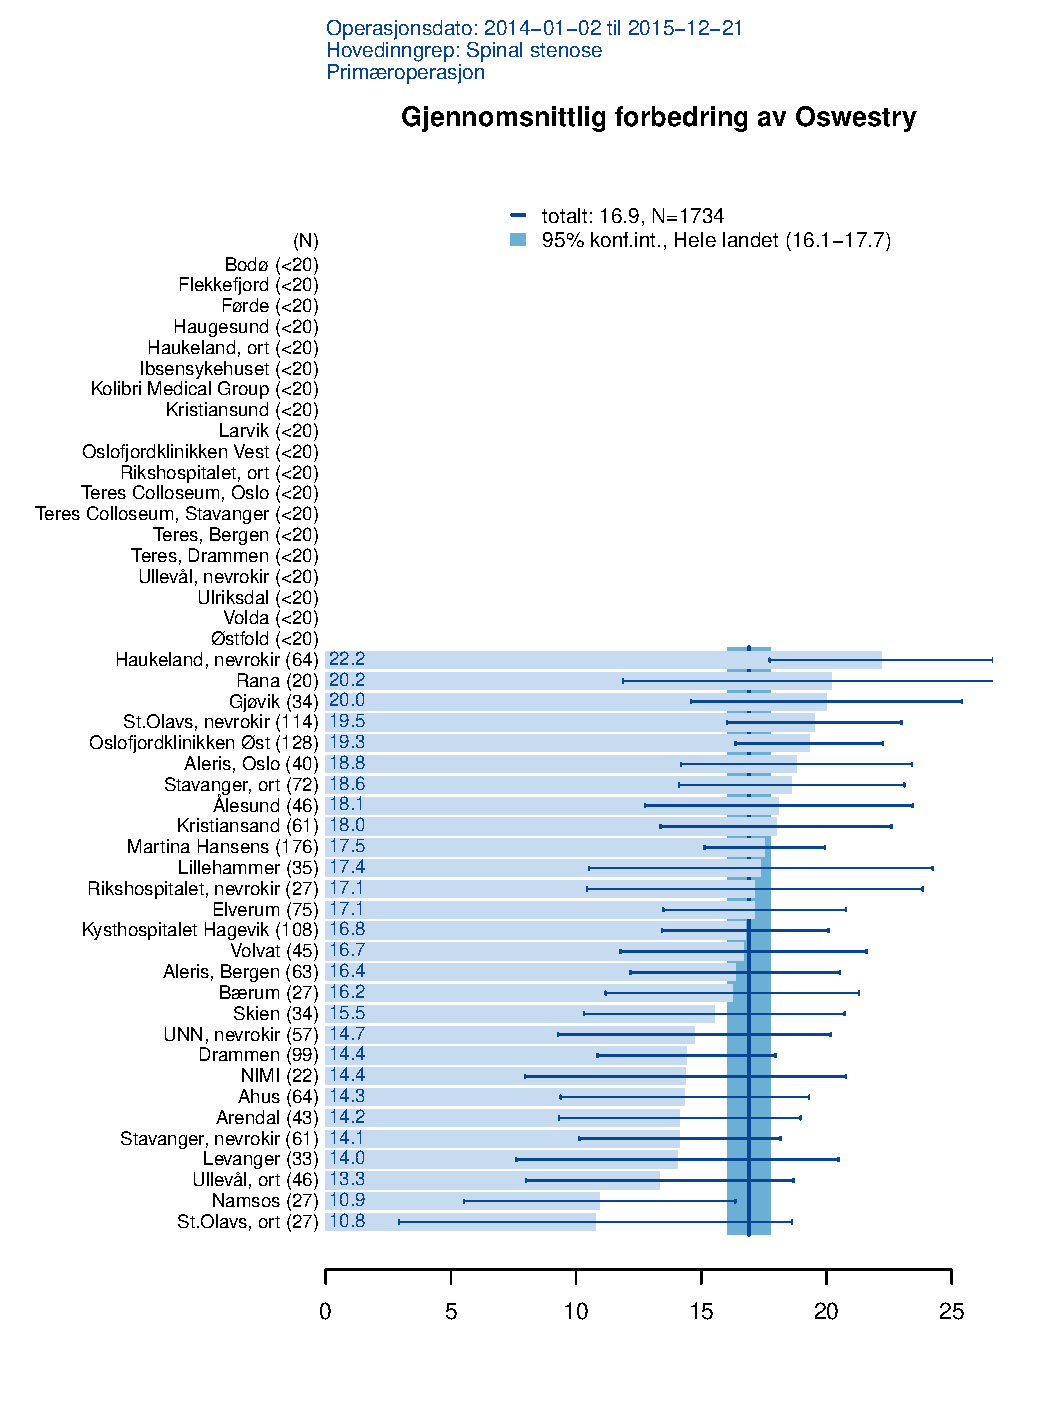
\includegraphics{Figurer/OswEndrAvdSS.pdf}}
\caption{Gjennomsnittlig endring av ODI per avdeling for spinal stenose.}
\label{fig:OswEndrAvdSS}
\end{figure}



\clearpage


ODI skår under eller lik 22 poeng oppleves av de fleste pasientene som et godt og helt akseptabelt fysisk funksjonsnivå 12 mnd etter ryggopersjon. Figurene \ref{fig:Osw22Pro} og \ref{fig:Osw22SS} angir hvor stor andel av henholdsvis prolaps og spinal stenose opererete som oppnår dette.

\begin{figure}[ht]
\scalebox{0.7}{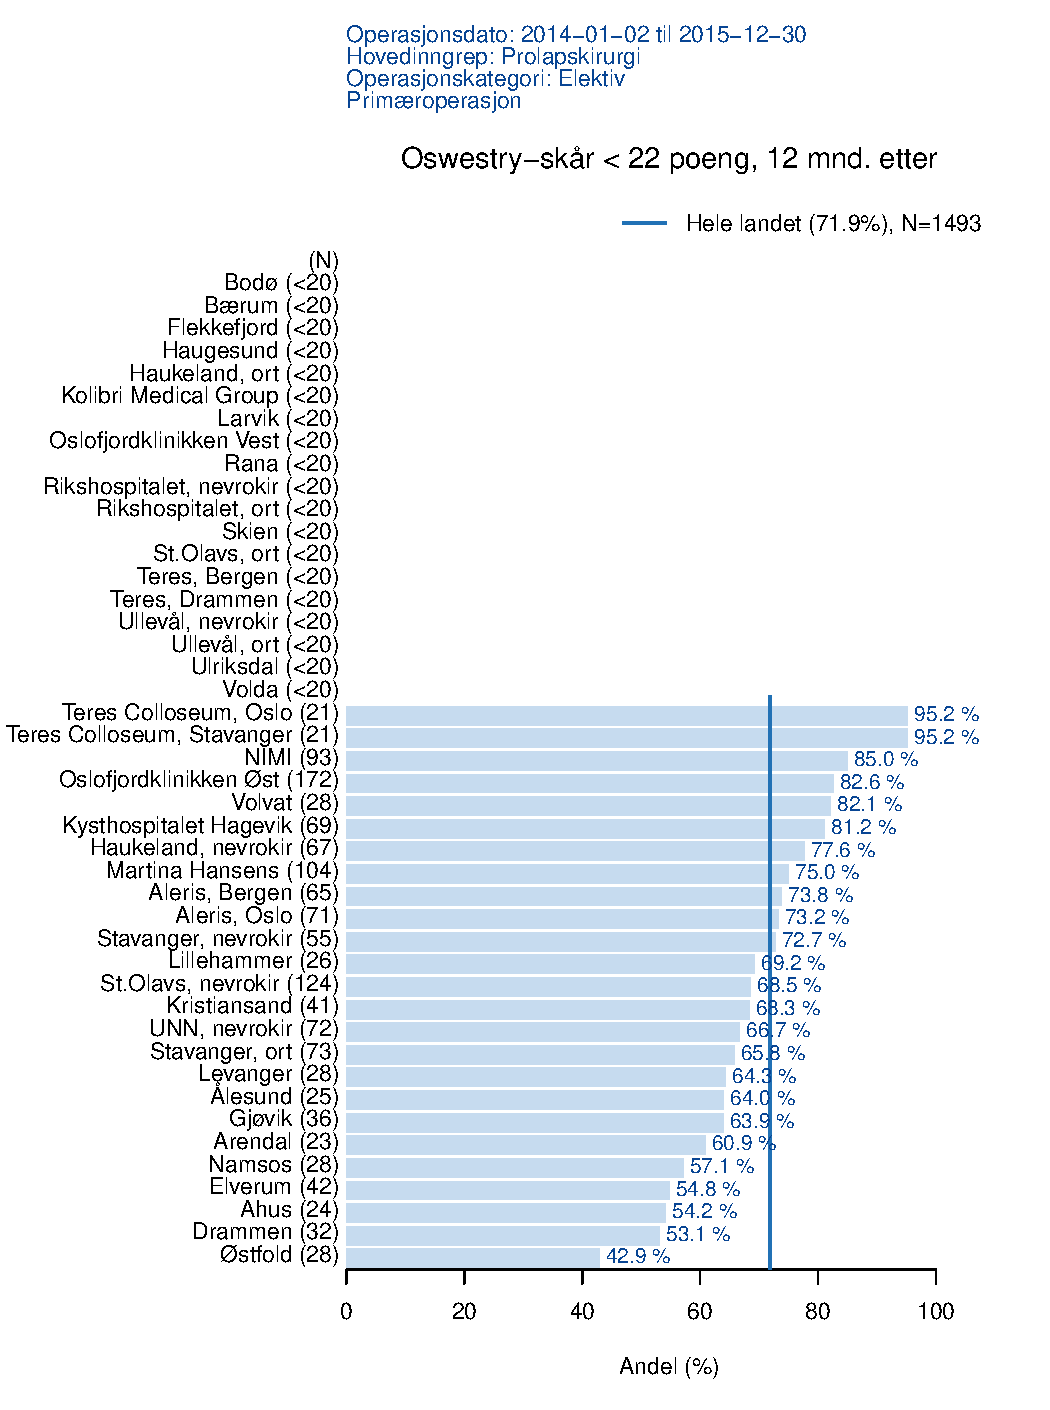
\includegraphics{Figurer/FigOsw22Pro.pdf}}
\caption{\label{fig:Osw22Pro}   Andel pasienter med ODI under 22 ett år
      etter prolapsoperasjon. Pasienter operert i 2015 og 2016.}
\end{figure}

\begin{figure}[ht]
\scalebox{0.7}{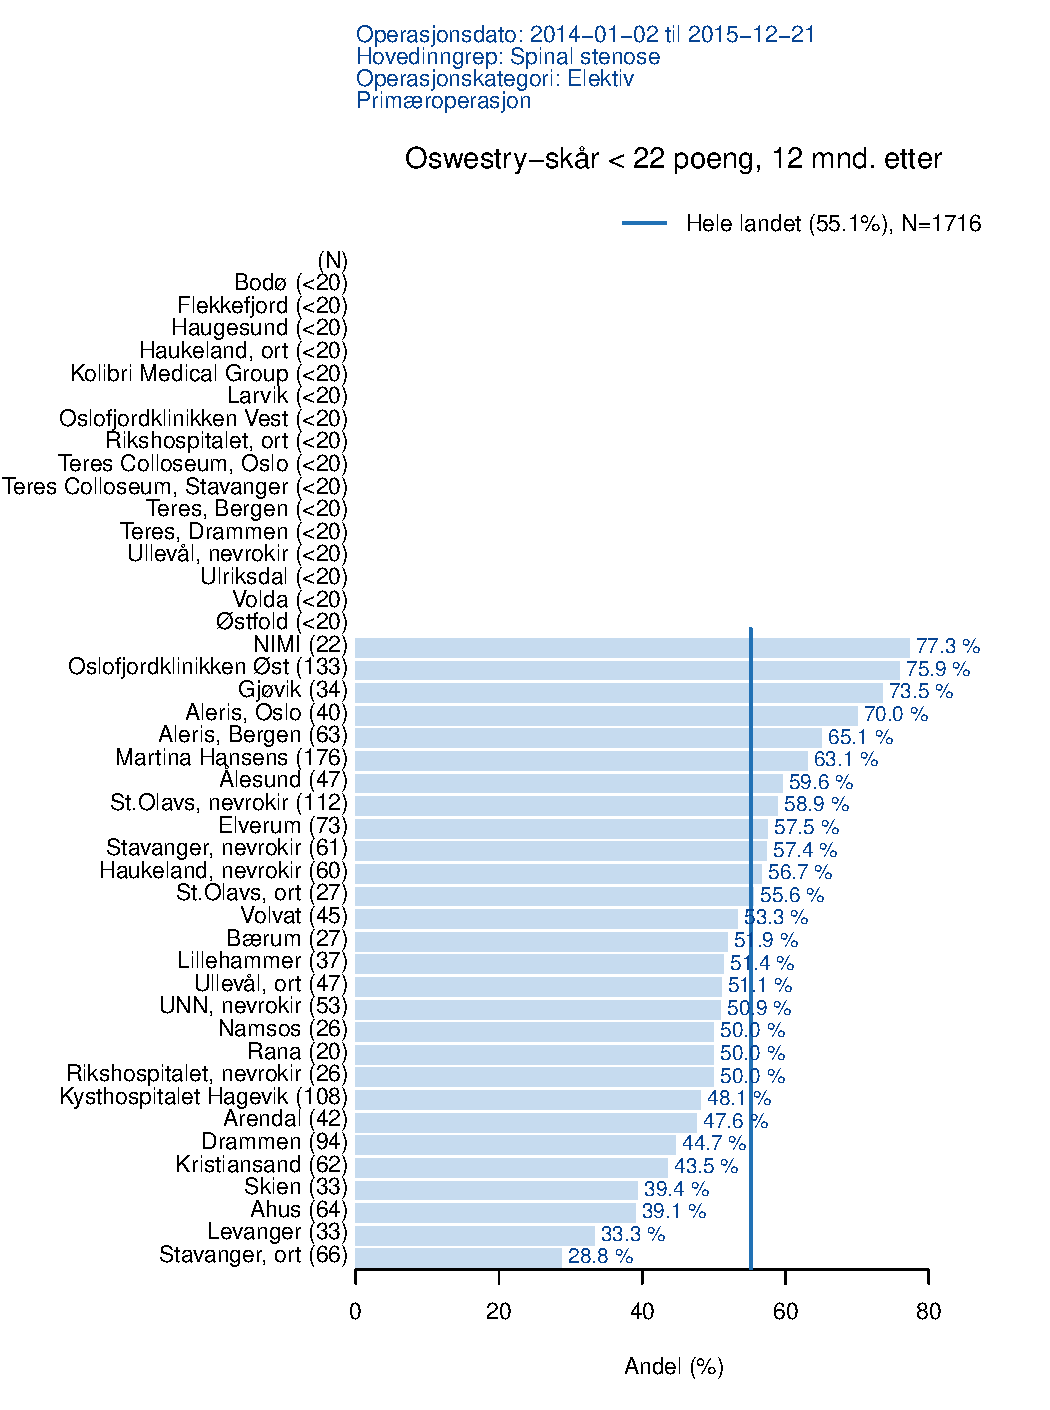
\includegraphics{Figurer/FigOsw22SS.pdf}}
\caption{\label{fig:Osw22SS}   Andel pasienter med ODI under 22 ett år
      etter spinal stenose operasjon. Pasienter operert i 2015 og 2016.}
\end{figure}


\clearpage

\subsection{Opplevd nytte av operasjon}
På spørreskjema etter operasjon blir pasientene bedt om å si hvor stor nytte de har hatt av operasjonen.
% De syv svaralternativene er angitt nedenfor og vår vitenskapelig baserte tolkinig er i parentes:
      % \begin{itemize}
% \item ''helt bra'' og ''mye bedre'' (Klart bedre)
% \item ''litt bedre'', ''ingen endring'' og ''litt verre'' (uendret) 
% \item ''mye verre'' og ''verre enn noen gang før'' (klar verre)
% \end{itemize}
Andelen som opplever at de har blitt helt bra eller mye bedre ett år etter operasjon har ligget stabilt siden 2011 og var 74\% for lumbalt prolaps og 60\% for spinal stenose opererte (2017) . Andelen  som angir at de er klart verre er henholdsvis har ligget stabilt rundt 3,0 \% for lumbalt prolaps og 5,5 \% spinal stenose opererte.
Et viktig fokusområde for NKR er å redusere andelen ryggopererte som får et dårlig operasjonsresultat.



      
      % \begin{figure}[h] 
% \begin{center}
% \scalebox{s2}{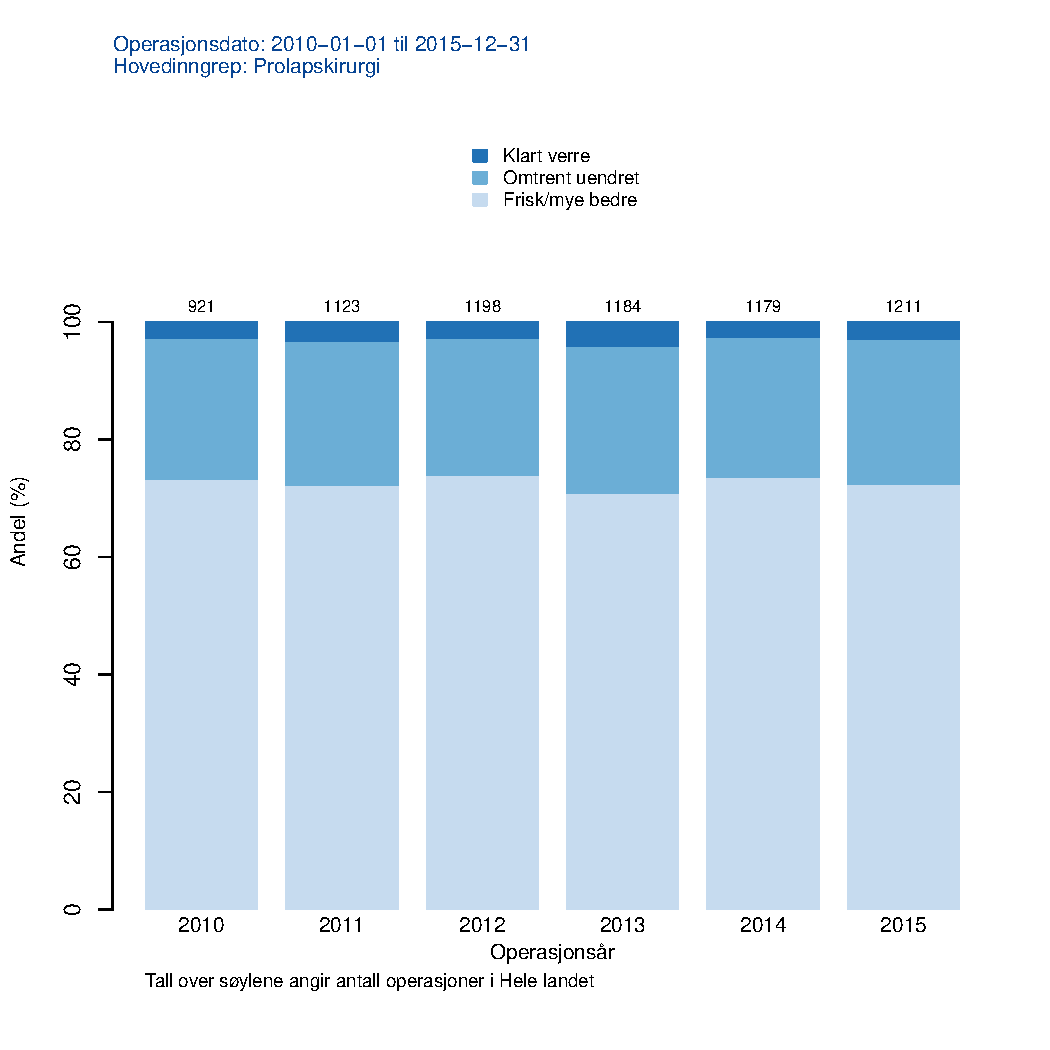
\includegraphics{Figurer/FigNyttePro.pdf}}
% \scalebox{s2}{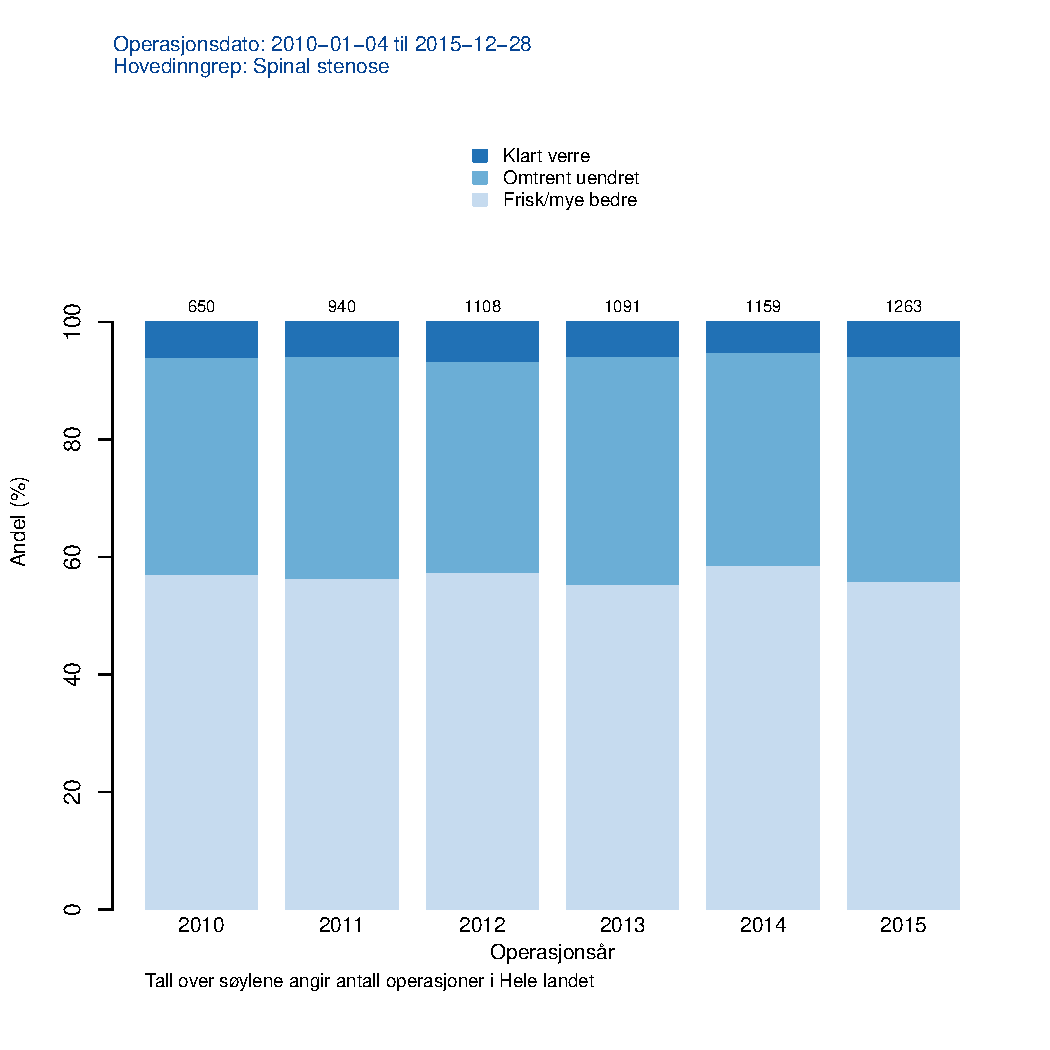
\includegraphics{Figurer/FigNytteSS.pdf}}
% \end{center}
% \caption{Spørsmål stilt 12 måneder etter operasjon til henholdsvis prolaps- og spinal stenosepasienter$:$ Hvilken nytte mener du at du har hatt av operasjonen?}
% \label{fig:Nytte}
% \end{figure}

\subsection{Pasienttilfredshet (PREM)}

% Figur \ref{fig:Fornoyd} viser hvor fornøyde pasientene var med behandlinga de fikk på sykehuset ktrtxt 
% etter operasjon fordelt på operasjonsår. Tallet øverst på søyla angir antall pasienter som har svart. 
På spørreskjemaet kan pasienten angi ett av 5 svaralternativer:
      \begin{itemize}
\item Fornøyd
\item Litt fornøyd
\item Hverken fornøyd eller misfornøyd
\item Litt misfornøyd
\item Misfornøyd
\end{itemize} 

 
Svarert på dette spørsmålet gjenspeiler et totalinntrykk og vil avhenge av en rekke andre faktorer enn selve den kirurgiske behandlingen. Andelen pasienter operert for lumbalt prolaps som ett år etter behandlinga er fornøyde med behandlingen de fikk på sykehuset  
ligger mellom 78 \% og 81 \% 
      for pasienter operert i perioden. 
%      startAar-rappAar. 
Tilsvarende ligger andel for lumbal spinal stenose ligger mellom 73 \% 
og 77 \%
Lumbal spinal stenose opererte gjennomgående var litt mindre fornøyd med behandlingen de fikk på sykehuset sammenliknet med prolapspasientene.





      
      % \begin{figure}[h] 
% \begin{center}
% \scalebox{s2}{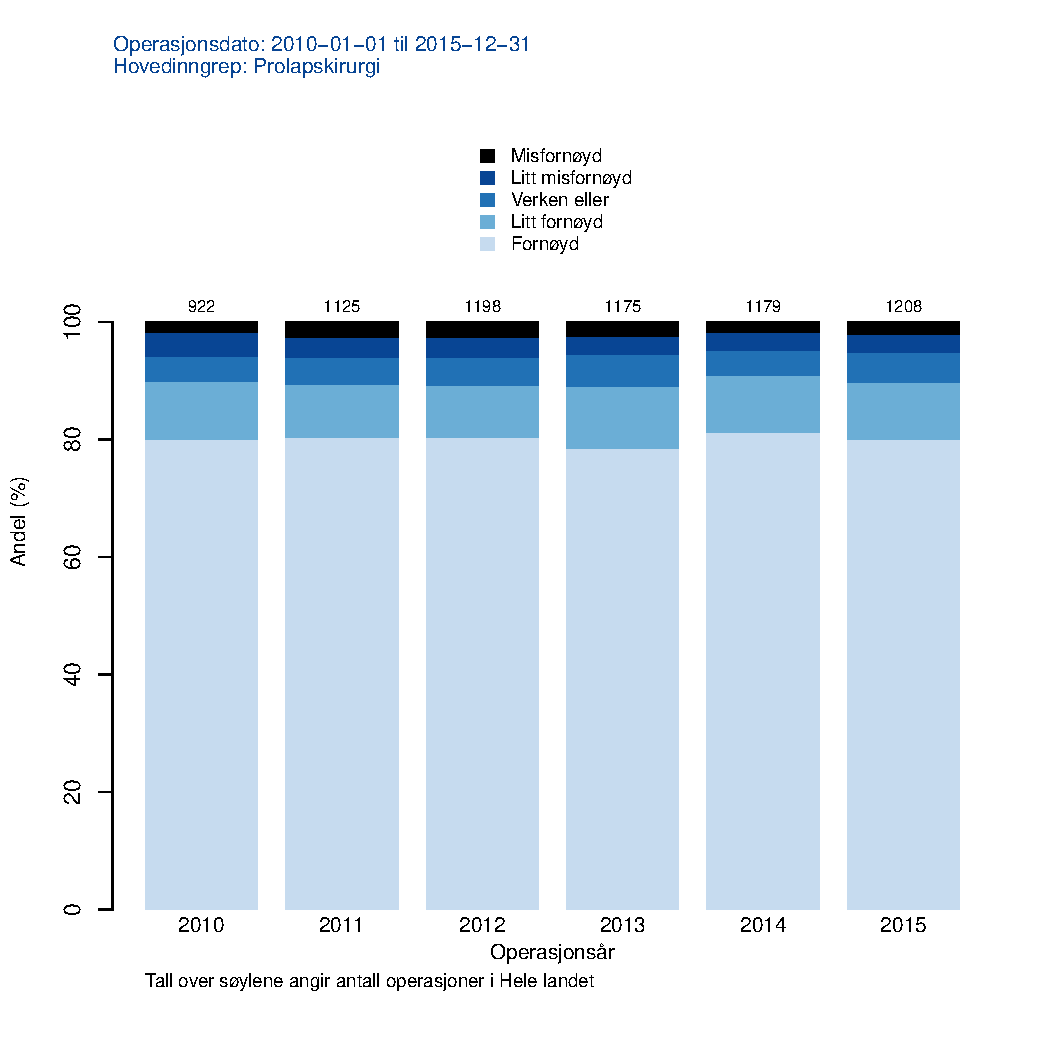
\includegraphics{Figurer/FigFornoydPro.pdf}}
% \scalebox{s2}{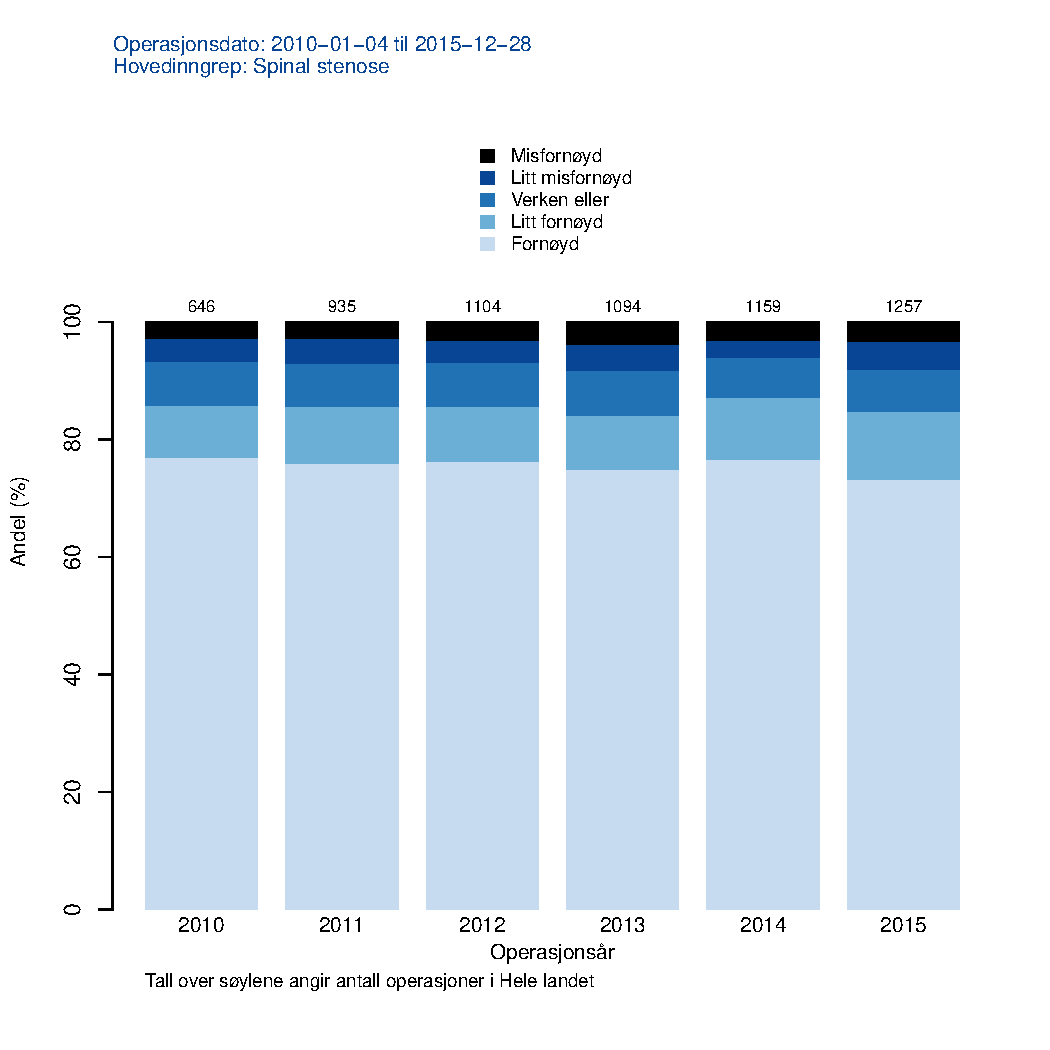
\includegraphics{Figurer/FigFornoydSS.pdf}}
% \end{center}
% \caption{Spørsmål stilt 12 måneder etter operasjon: Hvor fornøyd er du med behandlinga du har fått på sykehuset? til henholdsvis prolaps- og spinal stenosepasienter}
% \label{fig:Fornoyd}
% \end{figure}

\begin{figure}[h] 
\scalebox{0.7}{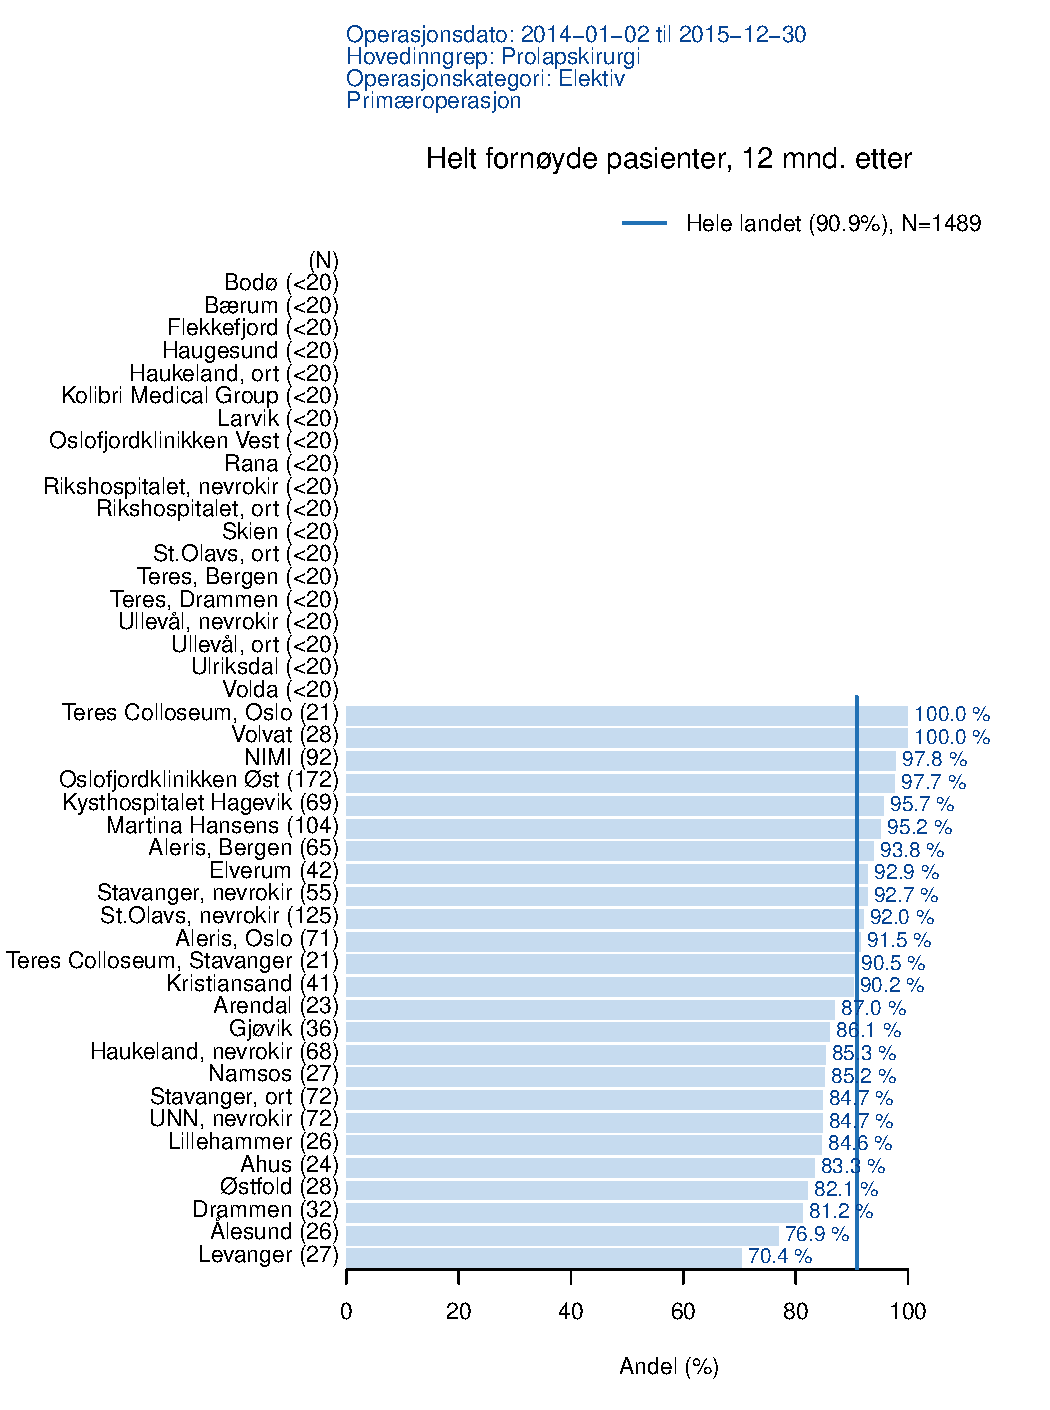
\includegraphics{Figurer/FigFornoydAvdPro.pdf}}
\caption{Andel pasienter operert for lumbalt prolaps i 2015 og 2016, som ett år etter er helt fornøyde med behandlinga de har fått på sykehuset}
\label{fig:FornoydAvdPro}
\end{figure}

\begin{figure}[h] 
\scalebox{0.7}{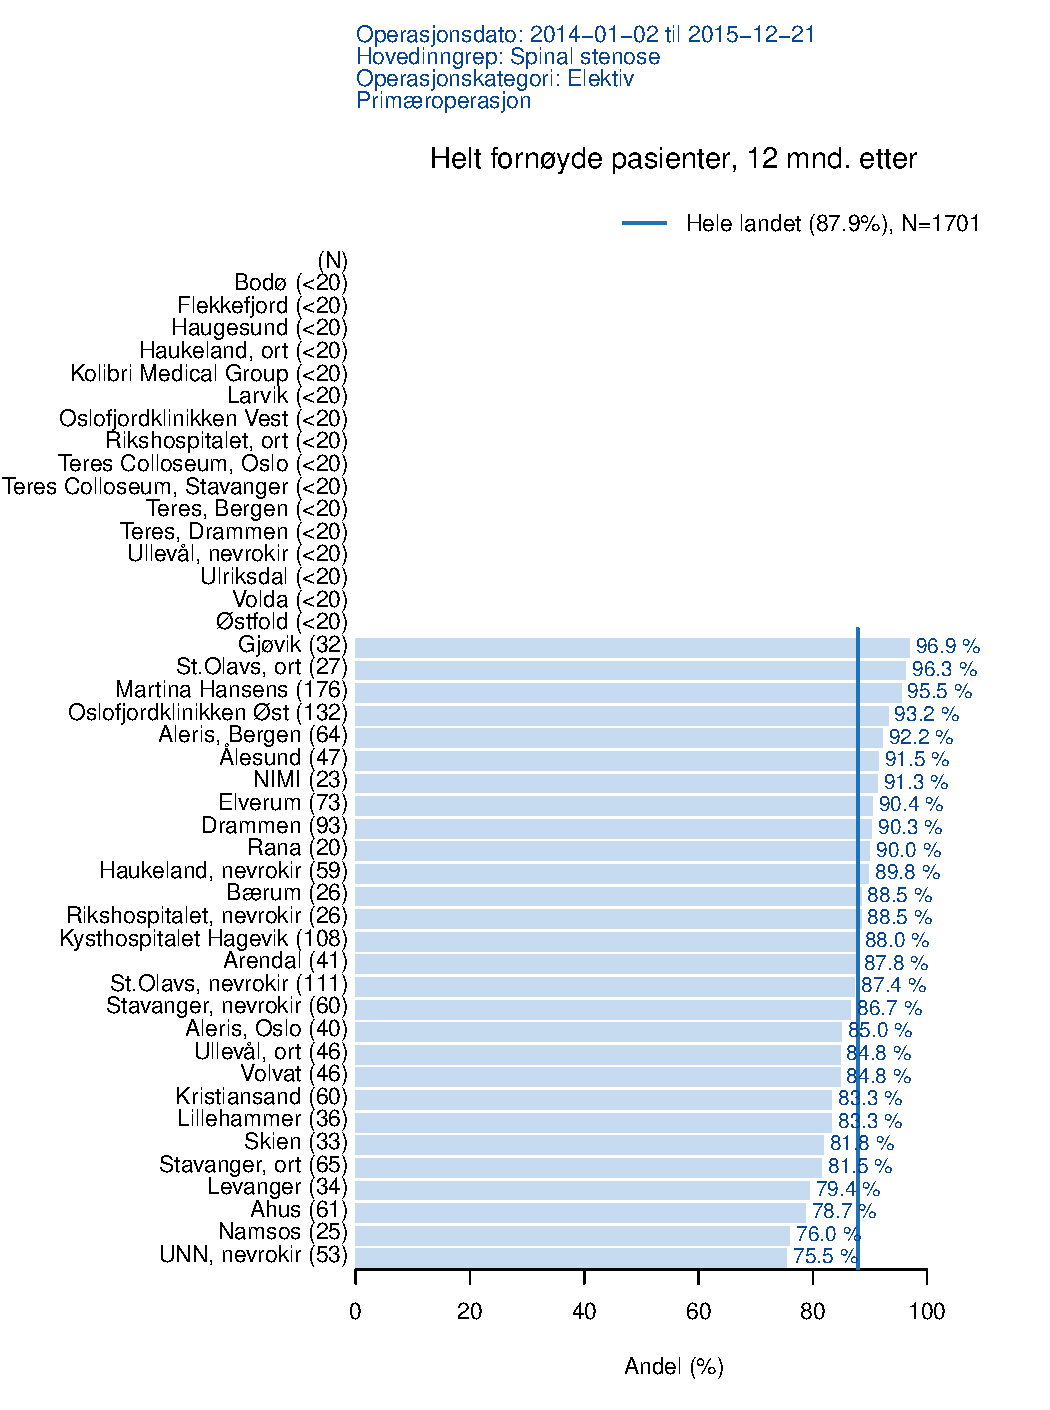
\includegraphics{Figurer/FigFornoydAvdSS.pdf}}
\caption{Andel pasienter opertert for lumbal spinal stenose i 2015 og 2016, som etter ett år er helt fornøyde med behandlinga de har fått på sykehuset}
\label{fig:FornoydAvdSS}
\end{figure}

\clearpage




      
      % Gjennomsnittlig liggetid på sykehus i forbindelse med prolapsoperasjon har gått ned med 
% NedgLiggetidPro døgn fra 2010 til rappAar.



\subsection{Kvalitetsindikatorer}
Det er viktig å merke seg at "indikator"  betyr en \textbf{mulig} sammenheng 
med kvalitet. Om indikatoren peker på et område som kan forbedres, må vurderes på det enkelte sykehus.

\subsubsection{Degenerativ rygg}



%\subsubsection{Sykehusvise resultater}


      
      Resultatene nedenfor gjelder planlagt, første gangs operasjon for lumbal spinal stenose og prolaps.
Kun avdelinger med mer enn 10 evt. 20 (avhenger av type resultat) registrerte operasjoner i er med i
analysen.
Grunnen til at reoperasjon og øyeblikkelig hjelp (ø-hjelp)
er filtrert bort er at andel slike inngrep er ulikt fordelt mellom sykehusene. 
      ''Suksess'' er her definert som mer enn 20 poengs forbedring av ODI. 
Hos pasienter med lumbalt prolaps som ikke har vært operert i ryggen tidligere er 
suksessraten 63.4 \% mot 54.8 \%. Hos prolapspasienter operert som ø-hjelp er andelen med betydelig forbedring 
(suksessrate)  78.7 \%, mot 57 \% av de som blir 
operert planlagt (elektivt). Dersom man har vært operert mer enn 2 ganger tidligere i
ryggen faller suksessraten fra  for lumbal spinal stenoseopererte betydelig (10\%). Langt færre pasienter i spinal stenosegruppen opereres som øyeblikkelig hjelp; 0.6 \%.  

Sykehus som får henvist få pasienter som ø-hjelp og
mange til reoperasjon vil dermed få dårligere resultater. 

 



For degenerativ rygg har fagrådet til NKR har valgt ut de kvalitetsindikatorerne som er angitt i tabell \ref{tab:KvalInd}
i kapittel \ref{sec:regspe}. 

\subsubsection{Dekningsgrad (Strukturmål)}
Høy dekningsgrad er en forutsetning for å kunne drive kvalitetssikring av egen virksomhet. Dekningsgraden gjenspeiler de ulike sykehusenes evne til og interesse for å evaluere sine egne resultater.

\clearpage

\subsubsection{Symptomvarighet for operasjon (Prosessmål)} 

Andelen pasienter som har hatt beinsmerter mer enn ett år på
operasjonstidspunktet var uendret fra 2011 til 2017 (47\%). 
I nasjonale retningslinjer (2007) er det anbefalt å operere pasienter for lumbalt prolaps før
beinsmertene har vart for lenge, helst innen ett år. Derfor bør denne
pasientgruppen håndteres raskt og effektivt når beslutning om operasjon er tatt og
ikke-kirurgisk behandling har vært forsøkt. Data fra NKR og nyere forskning viser at
pasienter som opereres for prolaps og har hatt beinsmerter mer enn ett år har
dårligere prognose. 
Det er stor variasjon i varighet av beinsmerter hos pasienter som blir
operert ved ulike sykehus. Det har sannsynligvis sammenheng med ventetid for
utredning og operasjon og tilgjengelig operasjonskapasitet i forhold til etterspørsel.
Tabell  \ref{tab:Utstr} viser fordeling av hvor lenge pasientene har hatt utstrålende smerter. 



% latex table generated in R 3.5.0 by xtable 1.8-2 package
% Mon Oct 01 09:27:43 2018
\begin{table}[ht]
\centering
\begin{tabular}{lr}
  \hline
 & Andeler \\ 
  \hline
Ingen utstrålende smerter & 3\% \\ 
  $<$ 3 mnd & 12.4\% \\ 
  3 - 12 mnd & 35.1\% \\ 
  1 - 2 år & 18.7\% \\ 
  $>$ 2 år & 25.8\% \\ 
  Ikke besvart & 5.1\% \\ 
   \hline
\end{tabular}
\caption{Varighet av nåværende utstrålende smerter} 
\label{tab:Utstr}
\end{table}

      
      

Figurene \ref{fig:VarighSmerteUtstrAvdPro} og \ref{fig:VarighSmerteUtstrAvdSS} viser hvor stor andel av henholdsvis prolaps- og spinal stenosepasienter som har hatt ustrålende smerter i mer enn ett år ved hvert sykehus.

Det er bekymringsfullt liten reduksjon i symptomvarighet før kirurgi fra år til år, spesielt for gruppen som ble opereret for lumbalt prolaps.



 


\begin{figure}[h] 
\scalebox{0.7}{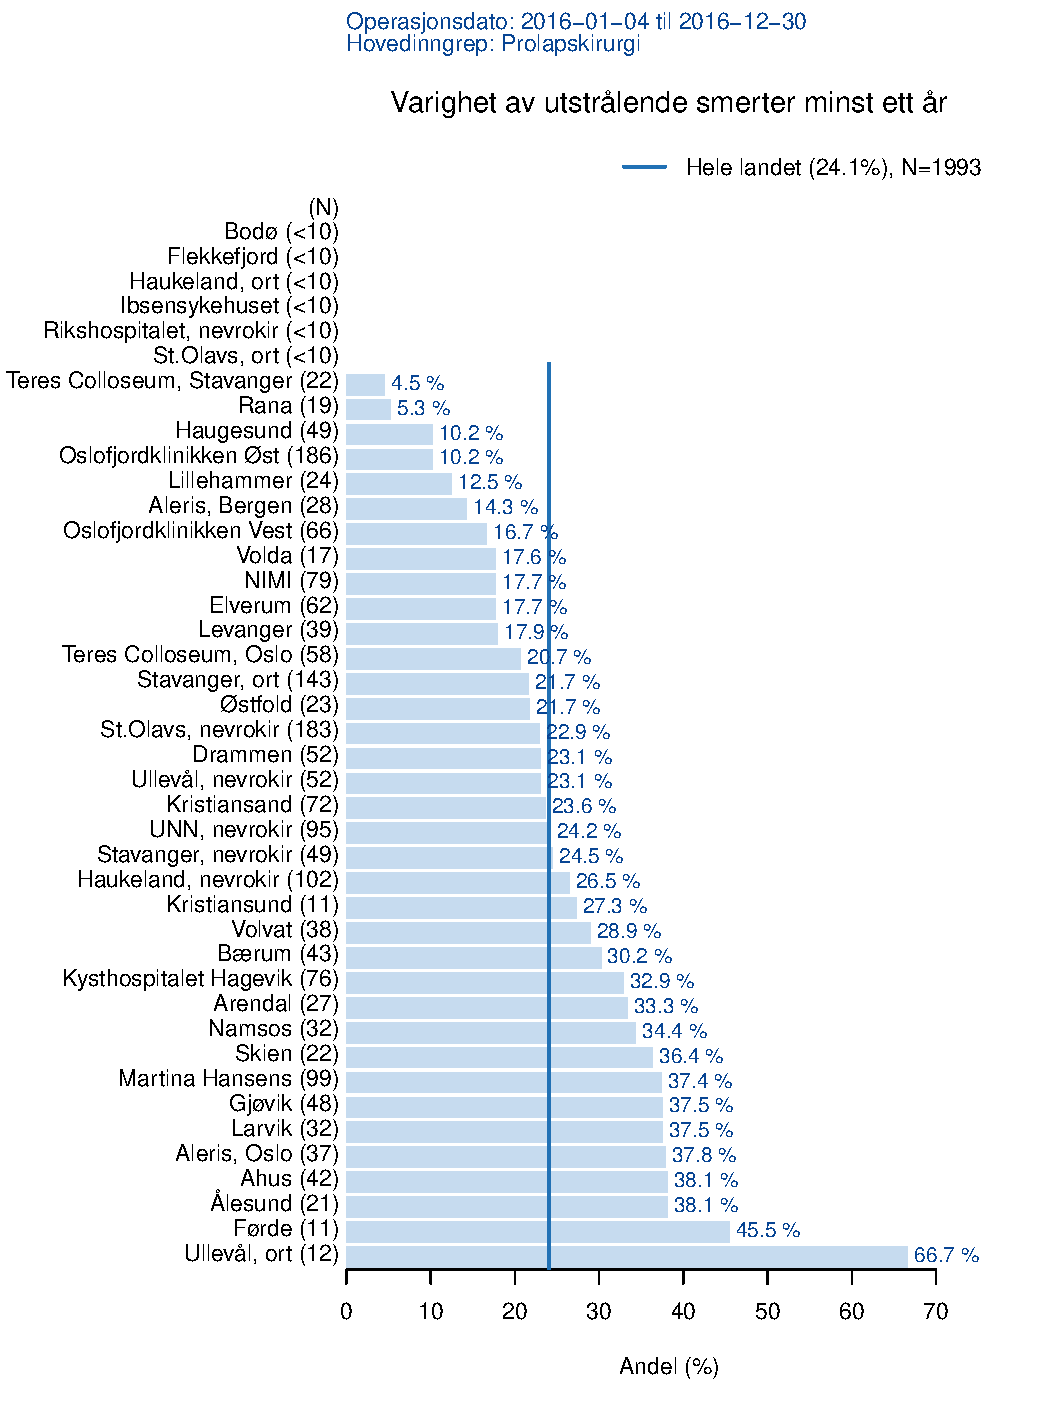
\includegraphics{Figurer/VarighUtstrAvdPro.pdf}}
\caption{Lumbale prolapspasienter som har hatt utstrålende smerter i mer enn ett år før operasjonen.}
\label{fig:VarighSmerteUtstrAvdPro}
\end{figure}

\begin{figure}[h] 
\scalebox{0.7}{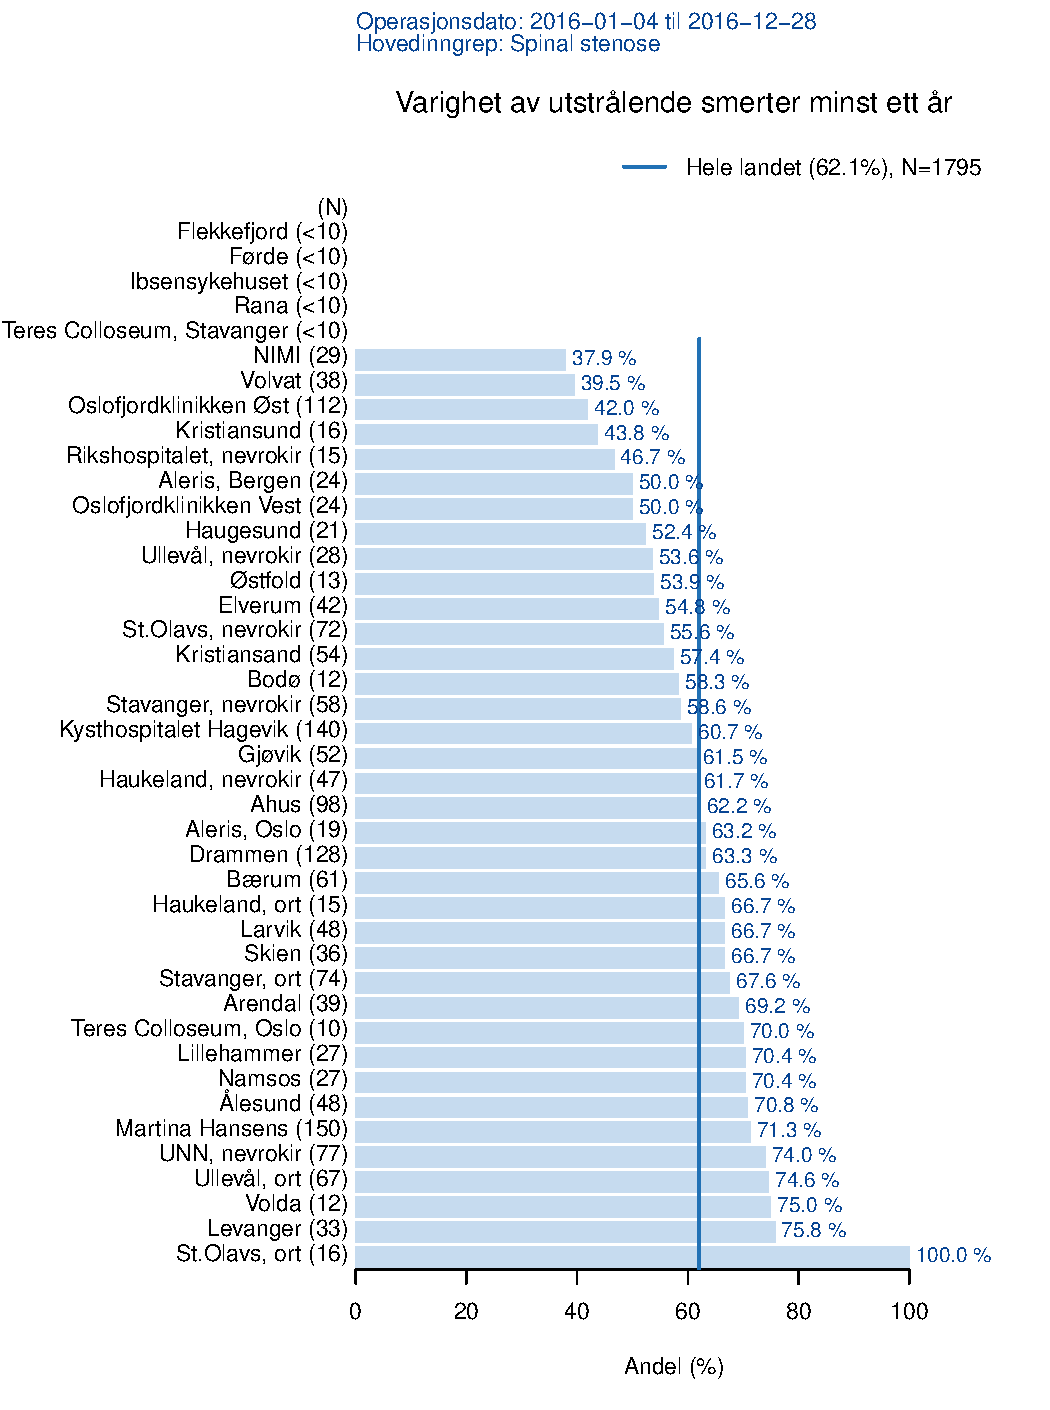
\includegraphics{Figurer/VarighUtstrAvdSS.pdf}}
\caption{Lumbal spinal stenosepasienter som har hatt utstrålende smerter i mer enn ett år før operasjonen.}
\label{fig:VarighSmerteUtstrAvdSS}
\end{figure}

Figur \ref{fig:VarighSmerteUtstrTid} viser utvikling over tid for andel pasienter med lang symptomvarighet. 

\begin{figure}[h] 
\center{
      \scalebox{0.55}{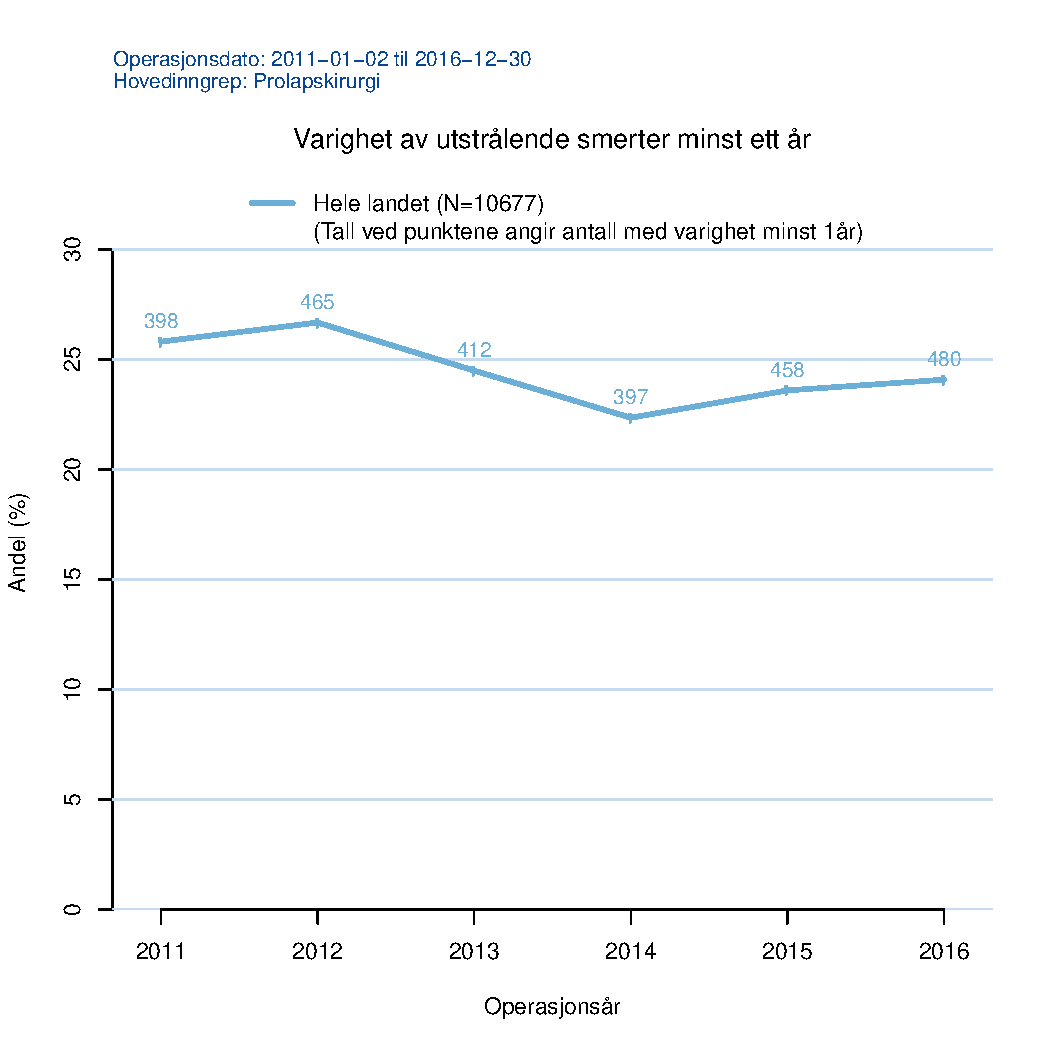
\includegraphics{Figurer/VarighUtstrTidPro.pdf}}
      \scalebox{0.55}{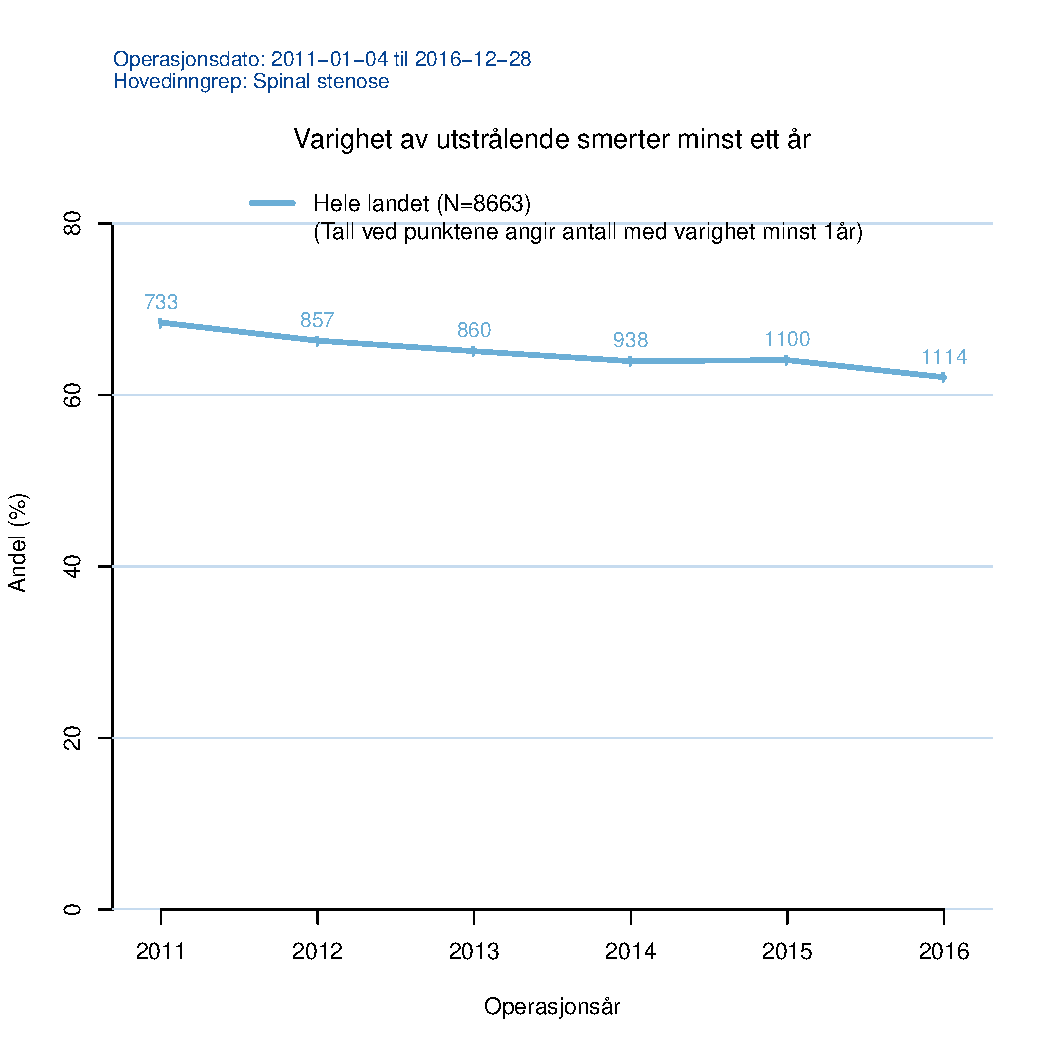
\includegraphics{Figurer/VarighUtstrTidSS.pdf}}} 
\caption{Prolaps- og Spinal stenosepasienter som har utstrålende smerter i mer enn ett år før operasjonen, utvikling over tid.}
\label{fig:VarighSmerteUtstrTid}
\end{figure}


%Lena: kun utstrålende smerter.

%\begin{figure}[h] 
%\scalebox{s1}{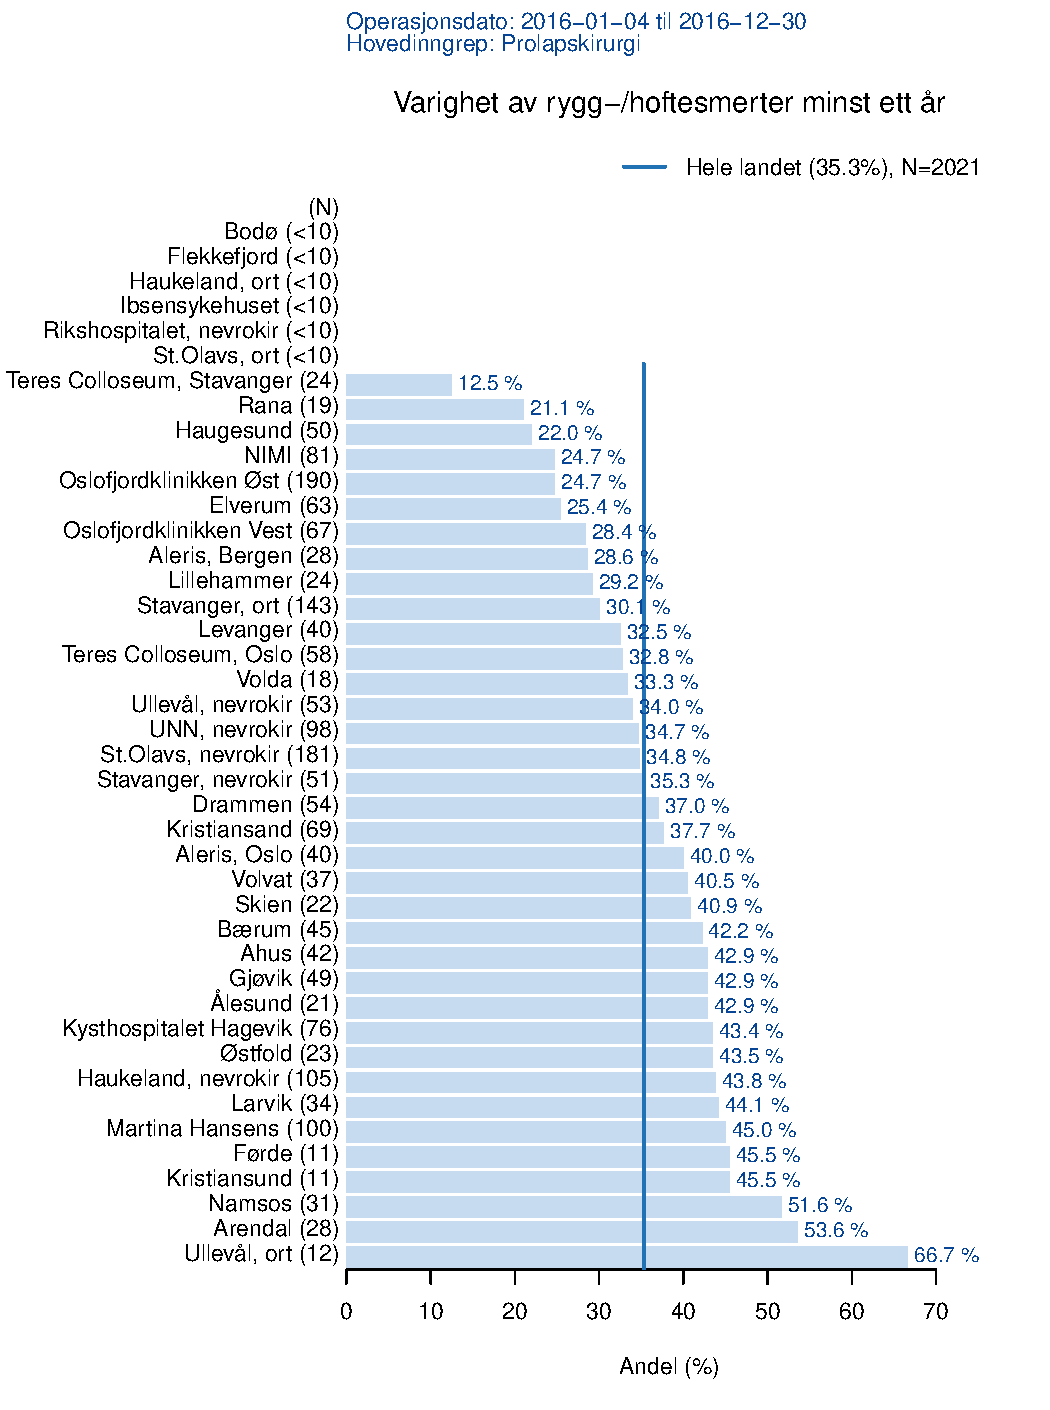
\includegraphics{Figurer/VarighRyggHofAvdPro.pdf}}
%\caption{Prolapspasienter som har hatt smerter i rygg-/hofte
      %i mer enn ett år før operasjonen.}
%\label{fig:VarighSmerteRyggAvdPro}
%\end{figure}

%\begin{figure}[h] 
%\scalebox{s1}{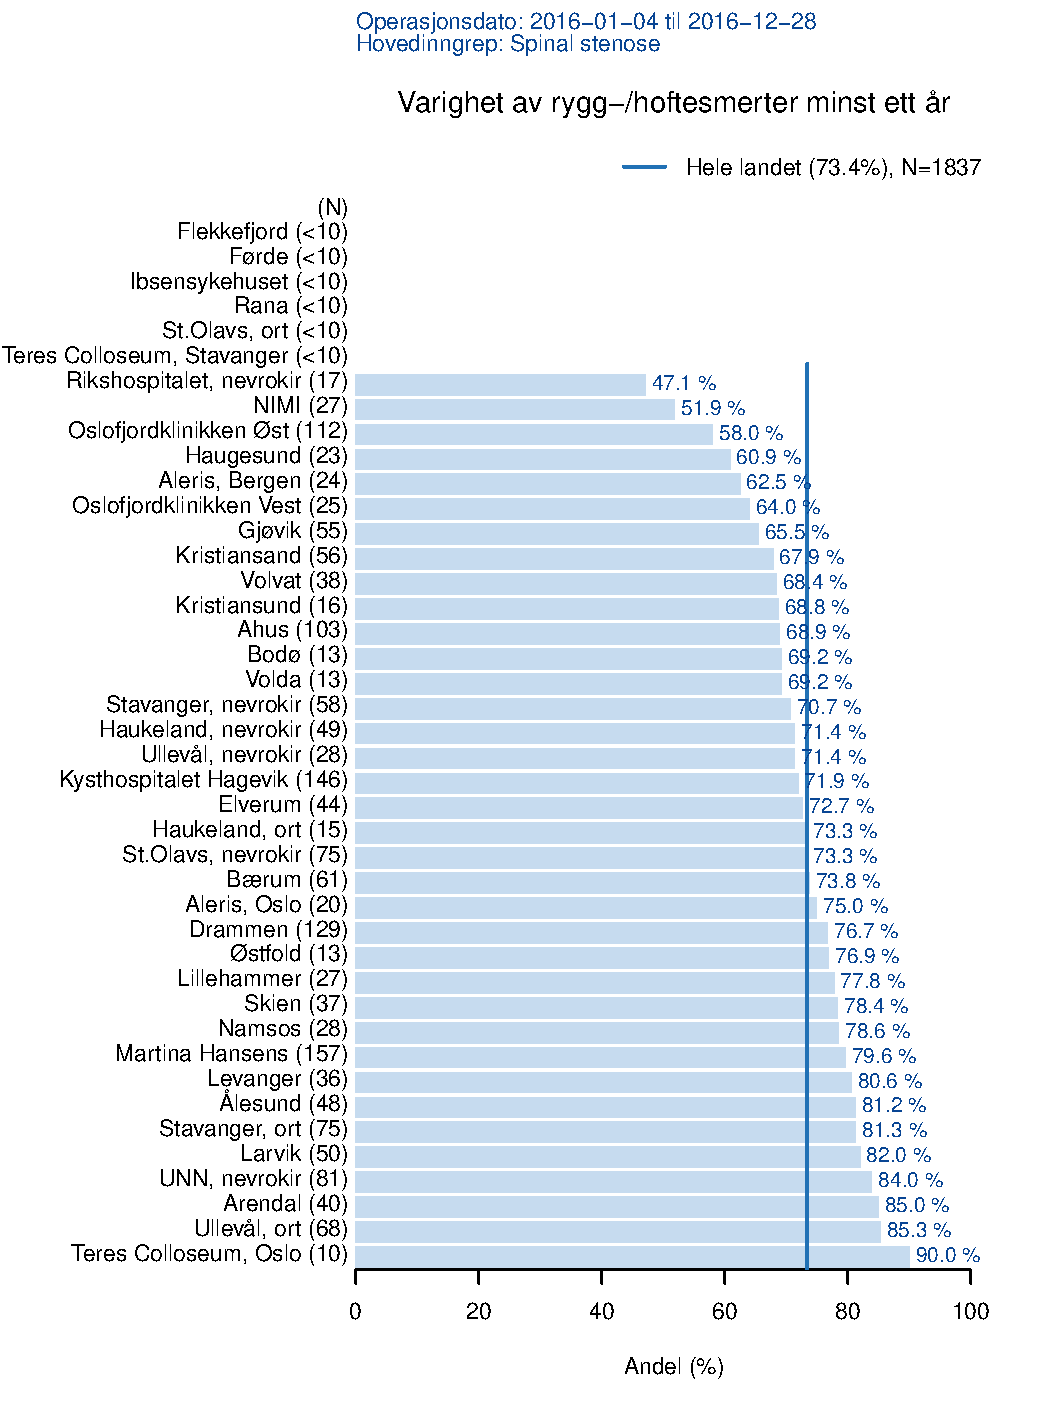
\includegraphics{Figurer/VarighRyggHofAvdSS.pdf}}
%\caption{Spinal stenosepasienter som har hatt smerter i rygg-/hofte
      %i mer enn ett år før operasjonen.}
%\label{fig:VarighSmerteRyggAvdSS}
%\end{figure}
									

\clearpage
 \subsubsection{Lite symptomer før operasjon (Prosessmål)}     
      Pasienter som har mye plager, vil kunne forvente størst nytte av ryggoperasjon,
mens de som har lite plager vil ha mindre potensial for forbedring og større risiko
for forverring. Gevinst av kirurgi henger derfor sammen med hvor streng
indikasjonsstillingen («inngangsbilletten» til kirurgi) har vært. Figur \ref{fig:BeinsmEndrPre} viser denne
sammenhengen tydelig. Det er verdt å merke seg er at hvis pasienten har lite smerter før
operasjon (bensmerter under eller lik 3 på den horisontale smerteskalaen), er det stor
sjanse for at pasienten faktisk blir verre  etter
operasjon (mindre enn 0 på den vertikale skalaen). \\

\begin{figure}[ht]
\scalebox{0.7}{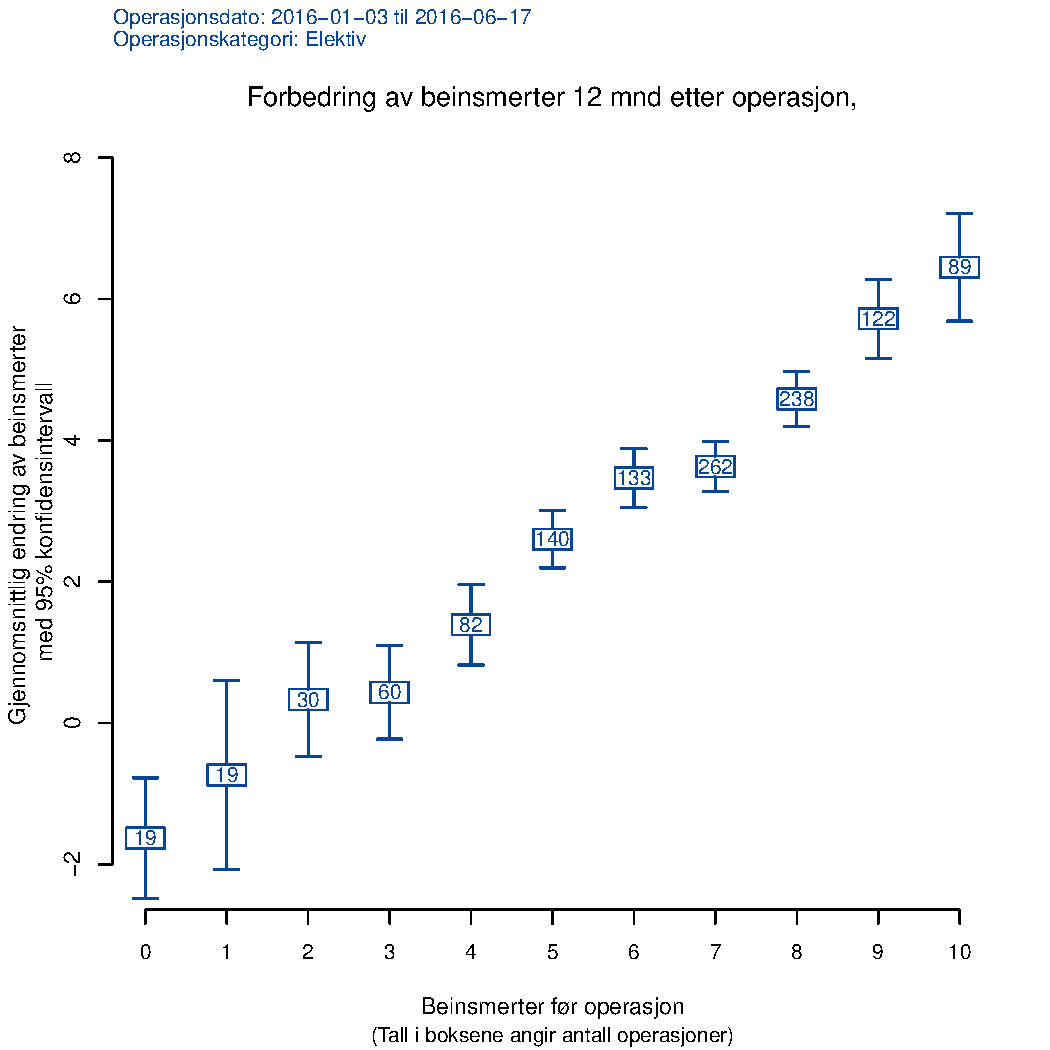
\includegraphics{Figurer/FigBeinsmEndrPre.pdf}}
\caption{\label{fig:BeinsmEndrPre}  Sammenheng mellom intensitet av bensmerte før operasjon og
      forbedring etter operasjon. Skala for bensmerter går fra 0 til 10, hvor 0 betegner
      ingen og 10 verst tenkelige smerte før operasjon (horisontal akse). Negativ endring
      av bensmerten (under 0 på vertikal akse) tilsvarer forverring, 0 betyr uendret smerte etter
      operasjon.}
\end{figure}

\clearpage

Figur \ref{fig:BeinsmLavPre} viser at det er stor variasjon i hvor stor grad sykehusene opererer
pasienter med lumbalt prolaps og lite beinsmerter . Pasienter med lammelse (parese) er tatt
ut av analysen, da de ofte må opereres uansett grad av smerte.




\begin{figure}[ht]
\scalebox{0.7}{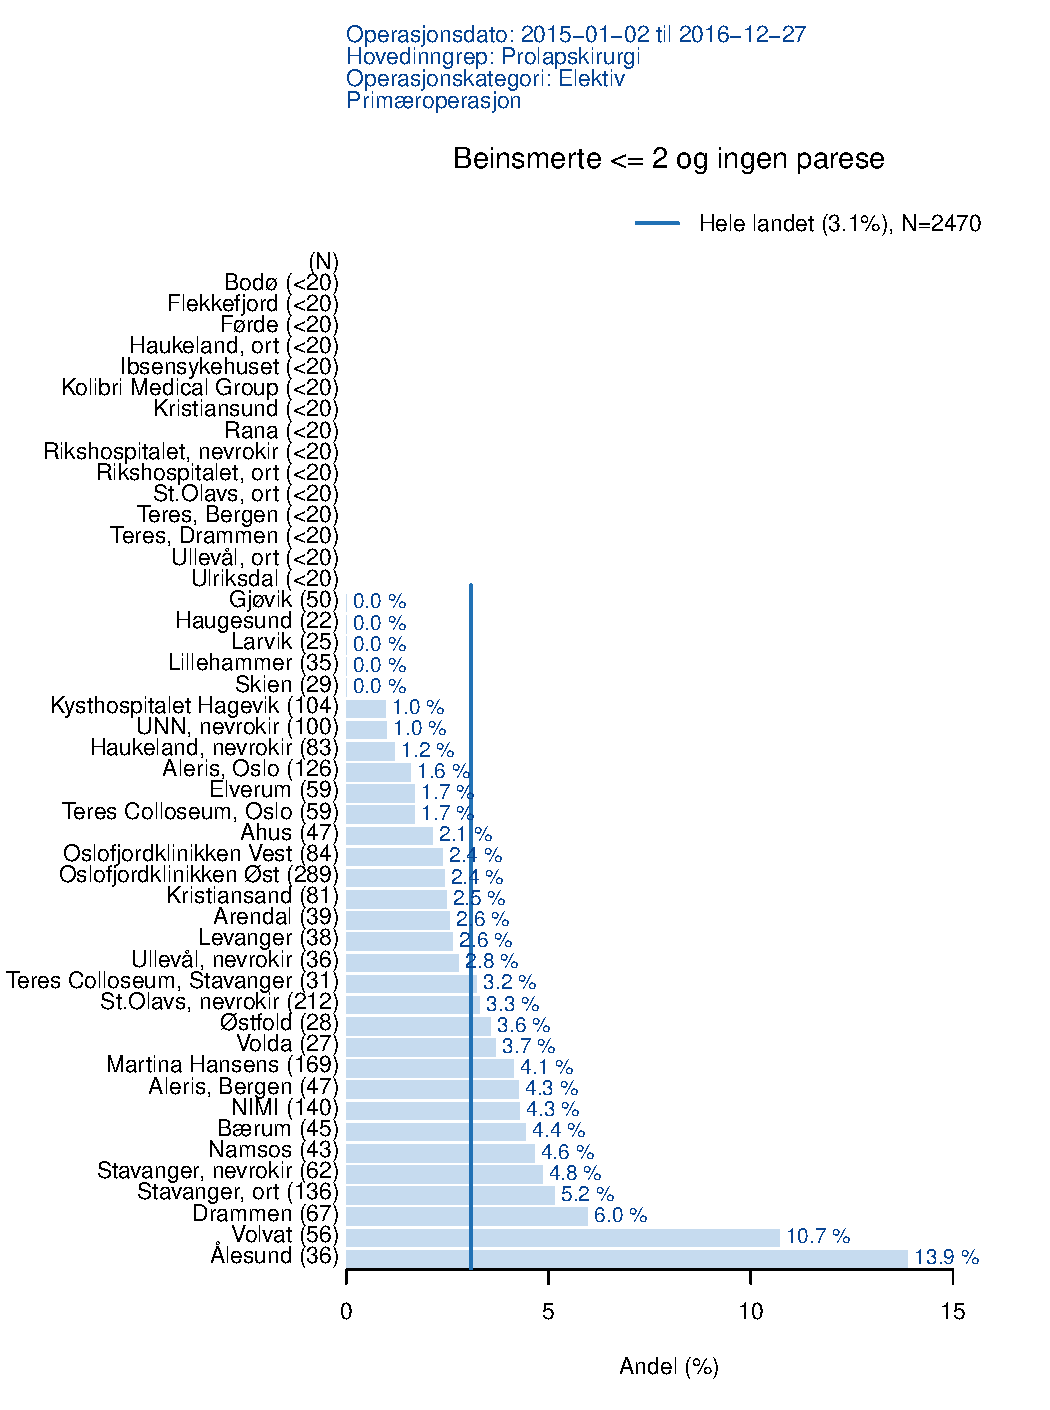
\includegraphics{Figurer/FigBeinsmLavPre.pdf}}
\caption{\label{fig:BeinsmLavPre}  Andel pasienter med lite beinsmerter ($\leq 3$) operert for prolaps siste to år.}
\end{figure}






\subsubsection{Sårinfeksjon (Resultatmål)}




\textbf{I. Sårinfeksjon.}

Årsakene til sårinfeksjoner er komplekse. NKR viste for mange år siden at dette har god forbyggende effekt. For lumbale prolaps operasjoner har
andel sårinfeksjoner (pasientrapportert) har blitt noe redusert fram til 2011, samtidig med at forbyggende antibiotikabehandling økte sterkt. I dag får 99\% antibiotika ved kirurgi for lumbalt prolaps og spinal stenose. Siden 2011 har andelen sårinfeksjoner ligget stabilt rundt 2 \% for prolapsopererte og rundt 3 \% for spinal stenose opererte.
Figurene \ref{fig:KpInfAvdPro} og \ref{fig:KpInfAvdSS} viser andel pasienter som fikk sårinfeksjon ved hver avdeling i årene 2016 og 2017.

      


%\begin{figure}[ht]
%      \centering \scalebox{s2}{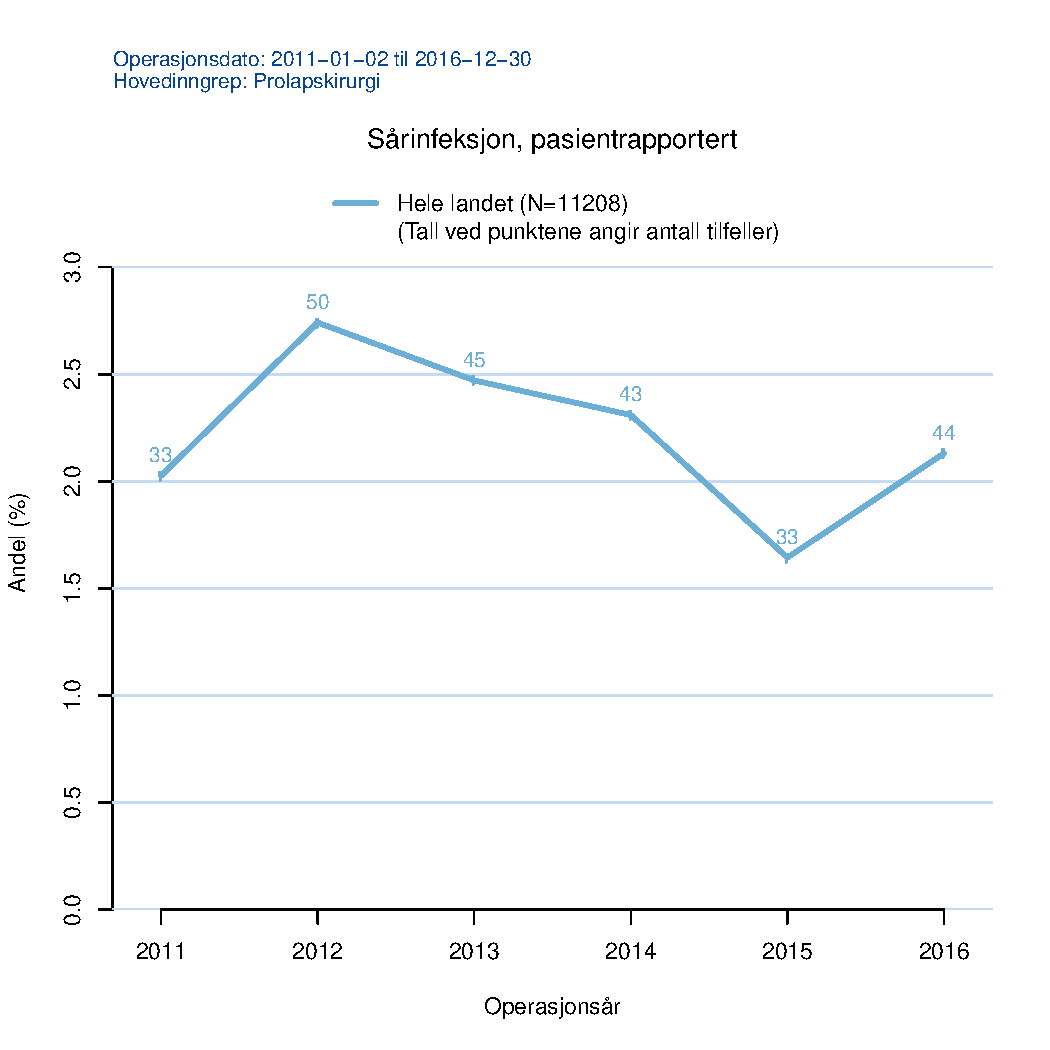
\includegraphics{Figurer/FigKpInf3MndTidPro.pdf}}
%      \centering \scalebox{s2}{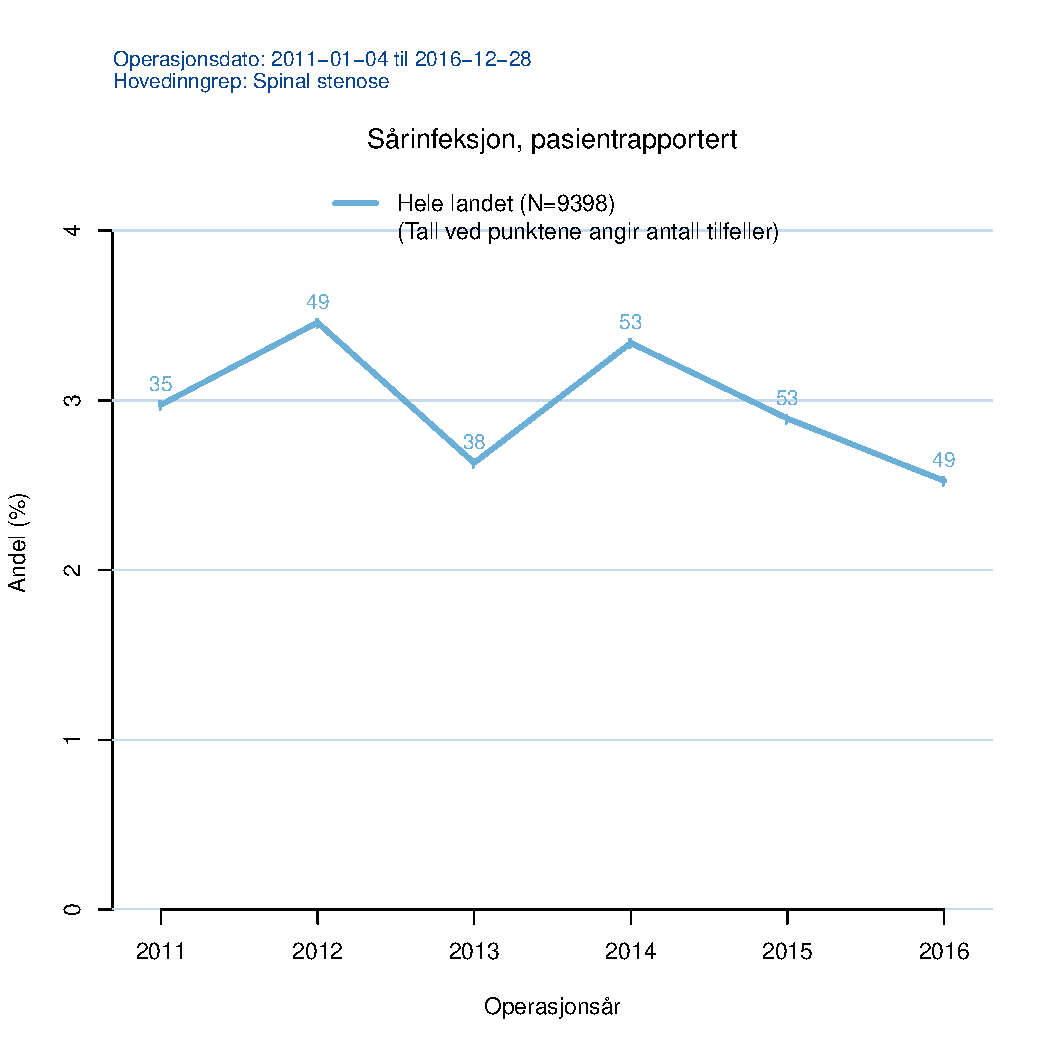
\includegraphics{Figurer/FigKpInf3MndTidSS.pdf}}
%      \caption{\label{fig:KpInfTid} Andel pasienter som rapporterer om sårinfeksjon 3 måneder etter
      %hhv. prolapskirurgi og spinal stenose, utvikling over tid.}
%\end{figure}



\begin{figure}[ht]
\scalebox{0.7}{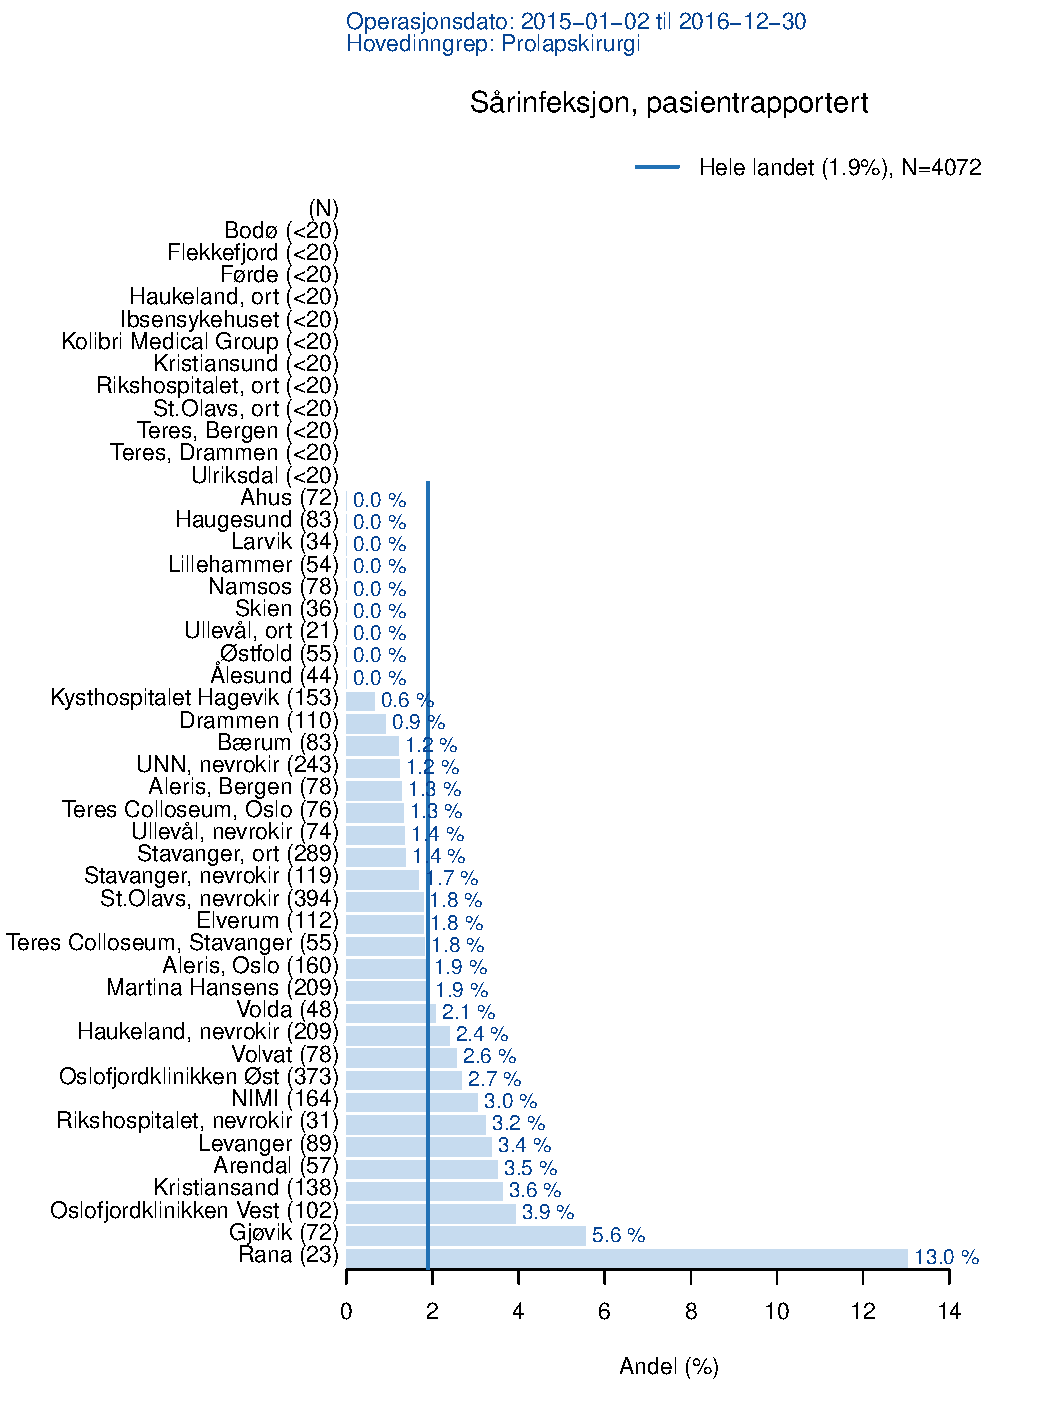
\includegraphics{Figurer/FigKpInf3MndPro.pdf}}
\caption{\label{fig:KpInfAvdPro} Andel pasienter som rapporterer om sårinfeksjon 
      (overfladisk og dyp) 3 måneder etter lumbal prolapskirurgi siste 2 år.}
\end{figure}

\begin{figure}[ht]
\scalebox{0.7}{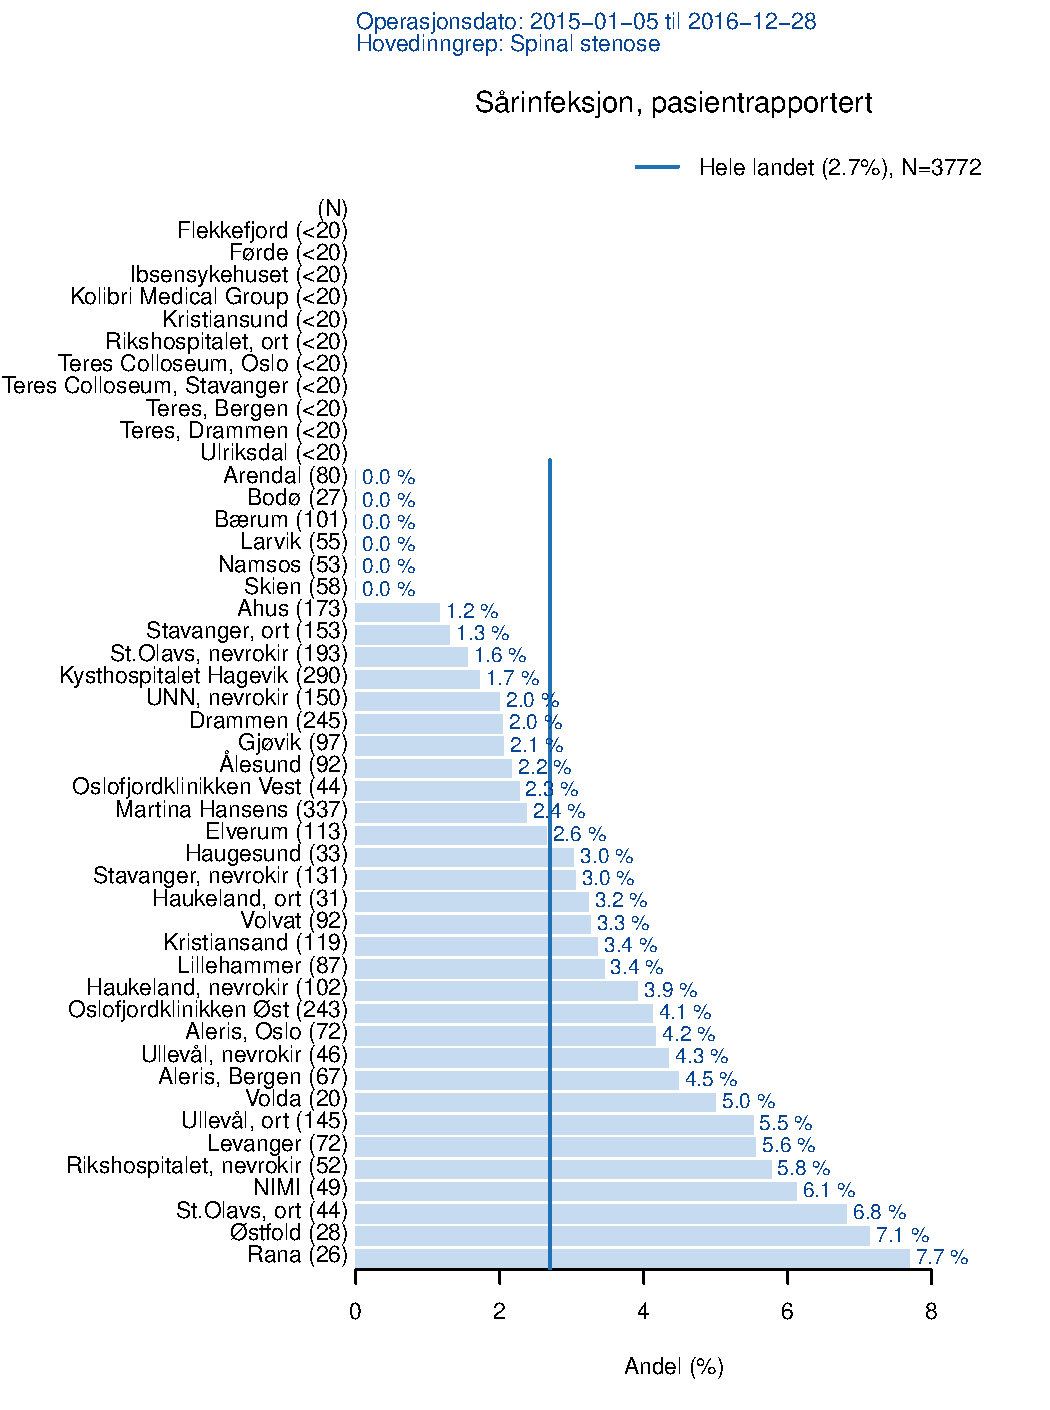
\includegraphics{Figurer/FigKpInf3MndSS.pdf}}
\caption{\label{fig:KpInfAvdSS} Andel pasienter som rapporterer om sårinfeksjon 
      (overfladisk og dyp) 3 måneder etter lumbal spinal stenose operasjon siste 2 år.}
\end{figure}

\clearpage

\subsubsection{Komplikasjoner (durarift)}


Durarift er oftest en ufarlig komplikasjon, men kan medføre væskelekkasje og
ubehag for pasienten, lengre liggetid og i noen tilfeller behov for reoperasjon.
Unntaksvis kan også konsekvensen være nerveskade og alvorlig infeksjon. Figurene \ref{fig:DuraPro} og \ref{fig:DuraSS} 
viser andelen som får durarift etter første gangs operasjon for henholdsvis lumbalt prolaps og spinal stenose i løpet av de 2 siste år.

\begin{figure}[ht]
\scalebox{0.7}{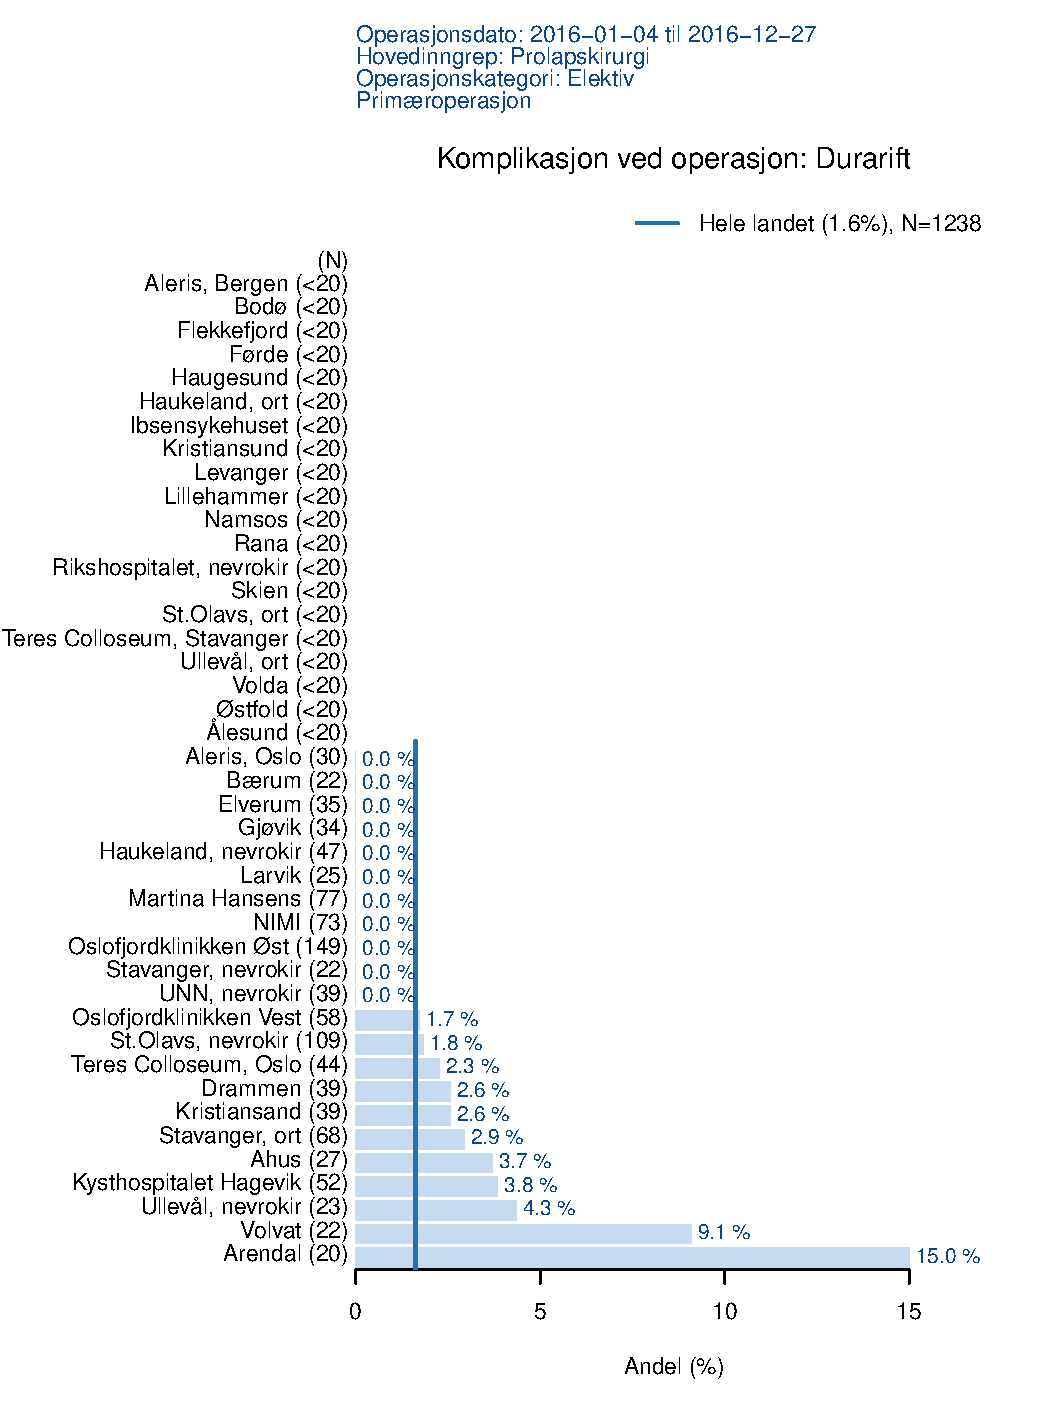
\includegraphics{Figurer/FigDuraPro.pdf}}
      \caption{\label{fig:DuraPro} Andel pasienter som fikk durarift etter kirurgi for lumbalt prolaps siste 2 år, 
      elektive pasienter, ikke tidligere ryggopererte.}
      \end{figure}
      
\begin{figure}[ht]
\scalebox{0.7}{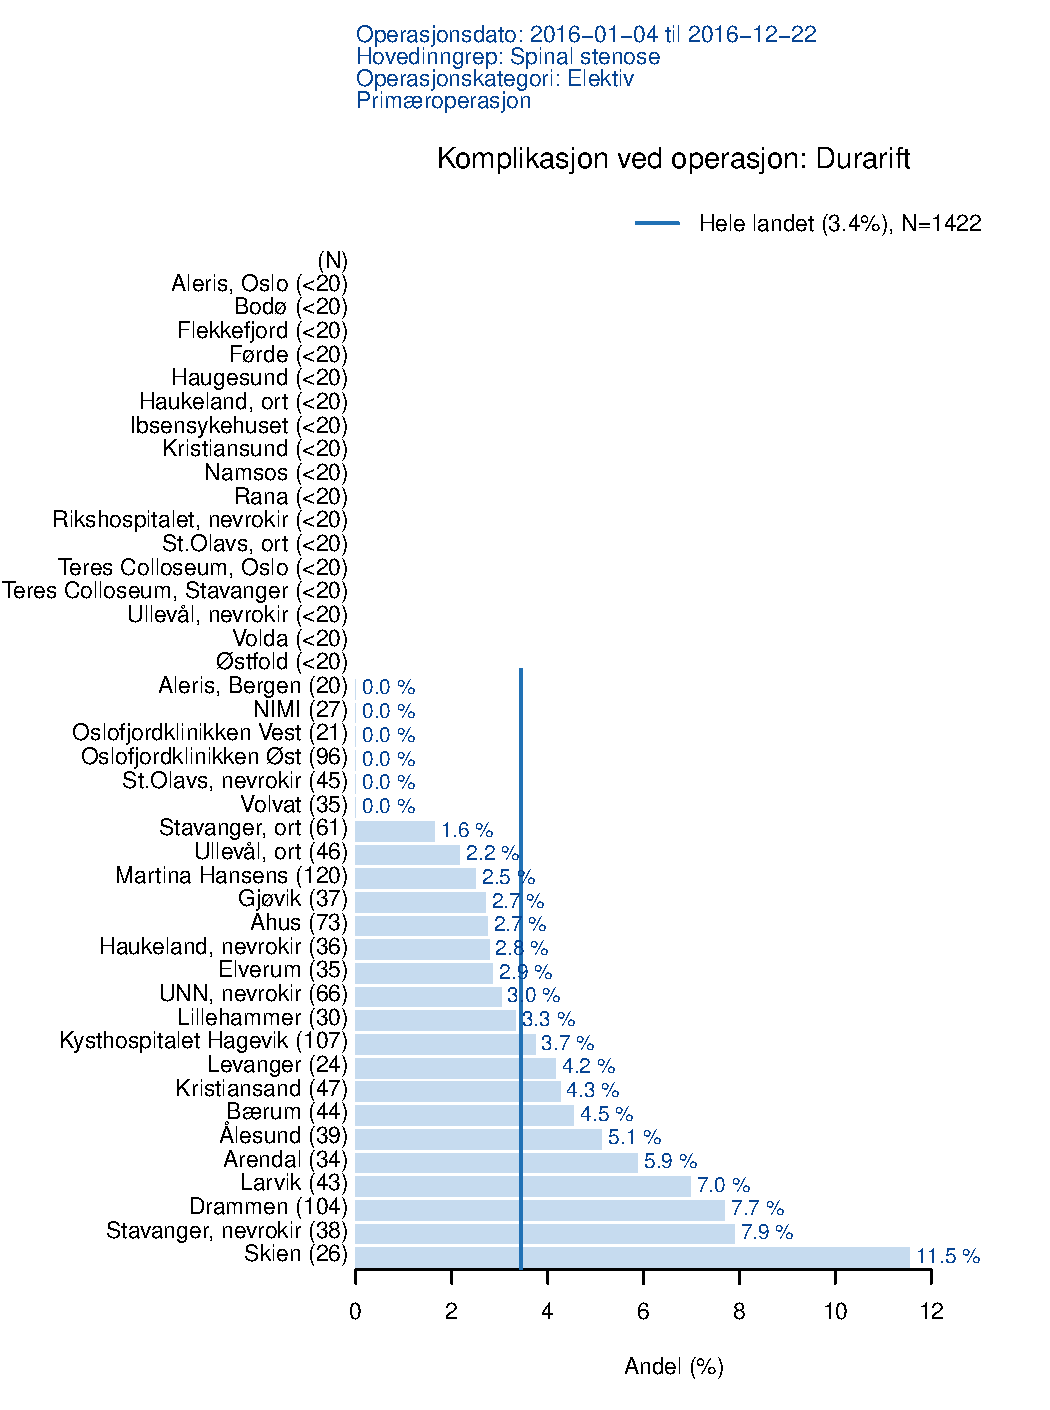
\includegraphics{Figurer/FigDuraSS.pdf}}
\caption{\label{fig:DuraSS} Andel pasienter som fikk durarift etter kirurgi for lumbal 
                  spinal stenose siste 2 år, elektive pasienter, ikke tidligere ryggopererte.}
\end{figure}

\clearpage



\section{Nakkekirurgi}

I Norge drives nakkekirurgi kun ved nevrokirurgiske avdelinger knyttet til de fem
universitetssykehusene i Oslo, Bergen, Trondheim, Stavanger og Tromsø, samt ved
hovedsakelig ett privat sykehus (Oslofjordklinikken).

Pasienter som opereres i nakken for degenerative tilstander har armsmerte med eller 
uten funksjonssvikt (radikulopati), varierende grad av nakkesmerter og noen har ryggmargspåvirkning (myelopati). 

Da  det ikke finnes nasjonale kvalitetsindikatorer for nakkekirurgi vil det bli en
viktig oppgave for NKR å utvikle slike i fremtiden. Det pågår derfor flere forskningsstudier i regi av NKR som ville kunne bidra til dette. 
Her presenteres sykehusvise data splittet på diagnose og behandling.




\subsection{Bakgrunnsdata, degenerativ nakke}


%\subsubsection{Alder, kjønn og komorbiditet}
Gjennomsnittsalder ved nakkeoperasjon var 52 år i 2017 og 84 \% ble operert med elektiv, planlagt kirurgi. Andel kvinner var  46 \%.
Andel som hadde ASA-grad over II var 9 \%. Andelen eldre over 70 år som nakkeopereres har ligget jevnt 
rundt 5 \% frem til og med 2017, men varierer noe mellom sykehus, spesielt mellom offentlige og private, 
Figur \ref{fig:NakkeAlder70Sh}.


\begin{figure}[ht]
\scalebox{0.65}{\includegraphics{Figurer/NakkeAlder70Sh.pdf}}
\caption{\label{fig:NakkeAlder70Sh} Andel nakkeopererte med alder over 70 år per sykehus siste år}
\end{figure}

\clearpage

\subsection{Virksomhetsdata}

Som hovedregel kan ikke pasienter som opereres på grunn av ryggmargspåvirkning (myelopati) påregne bedring etter kirurgi i motsetning til de som behandles for nerverotspåvirkning (radikulopati). Hensikten med å operere de som har ryggmargsskade er snarere å forhindre forverring. Figur \ref{fig:NakkeOprIndikMyelopatiSh} viser at andelen som opereres for myelopati varierer mellom sykehusene.

\begin{figure}[ht]
\scalebox{0.7}{\includegraphics{Figurer/NakkeOprIndikMyelopatiSh.pdf}}
\caption{\label{fig:NakkeOprIndikMyelopatiSh} Andel nakkeoperete med diagnosen myelopati siste år}
\end{figure}




\clearpage

\subsubsection{Sårdren}

Bruk av sårdren etter fremre nakkekirurgi har vært omdiskutert i litteraturen. Tidligere norske studier kan tyde på at bruk av sårdren er unødvendig, da det ikke ser ut til å redusere faren for postoperativ blødning. Figur \ref{fig:NakkeSaardrenUmFTid} viser at bruk av sårdren ved fremre nakkekirurgi er avtagende i Norge, men variasjonen mellom sykehus er stor, Figur \ref{fig:NakkeSaardrenUmFSh}.

\begin{figure}[ht]
\scalebox{0.7}{\includegraphics{Figurer/NakkeSaardrenUmFTid.pdf}}
\caption{\label{fig:NakkeSaardrenUmFTid} Andel som har hatt sårdren etter fremre nakkekirurgi i Norge per år.}
\end{figure}

\begin{figure}[ht]
\scalebox{0.7}{\includegraphics{Figurer/NakkeSaardrenUmFSh.pdf}}
\caption{\label{fig:NakkeSaardrenUmFSh} Andel som har hatt sårdren etter fremre nakkekirurgi per sykehus siste år.}
\end{figure}

\clearpage

\subsection{Resultatmål}

Pasientene er fulgt opp med spørreskjema 3 og 12 måneder etter kirurgi.
Resultatene er ikke justert for forskjeller i pasientpopulasjonene.

%\subsubsection{Sårinfeksjon}

\subsubsection{Resultat etter fremre nakkekirurgi for nerverotssmerte og funksjonssvikt (cervical radikulopati)}




Neck Disability Index (NDI) er et godt validert mål for å vurdere bedring i smerterelatert
funksjonshemming  i dagliglivets aktiviteter samt sykdomsspesifikk livskvalitet hos 
nakkeopererte. Til å måle armsmerteintensitet før og etter operasjon brukes numerisk 
smerteskala (NRS, 0-10). Figurene nedenfor viser resultater etter fremre nakkekirurgi hos 
pasienter som har nerverotssmerte og funkssjonsvikt (radikulopati) uten tegn til 
ryggmargsskade 
(myelopati). Figur \ref{fig:NakkeNRSsmerteArmEndr12mndUmFSh} og  
\ref{fig:NakkeNDIendr12mndUmFSh} at viser at mellom 60 og 70 \% har en betydelig forbedring av 
armsmerte og funksjonssvikt (NRS og NDI reduksjon tilsvarende 30 \%  eller mer) ett år etter 
kirurgi. Det et er variasjon i resultater mellom sykehus. Over 80 \% av pasientene er fonøyde 
med behandlingen de fikk, Figur \ref{fig:NakkeFornoydBeh12mndFremSh}.  





\begin{figure}[ht]
\scalebox{0.6}{\includegraphics{Figurer/NakkeNRSsmerteArmEndr12mndUmFSh.pdf}}
\caption{\label{fig:NakkeNRSsmerteArmEndr12mndUmFSh} Andel som har fått betydelig bedring av nerverotsmerte  etter fremre nakkekirurgi, siste 2 år.}
\end{figure}

\begin{figure}[ht]
\scalebox{0.7}{\includegraphics{Figurer/NakkeNDIendr12mndUmFSh.pdf}}
\caption{\label{fig:NakkeNDIendr12mndUmFSh} Andel pasienter som har fått betydelig bedring av fysisk funksjon i dagliglivet etter fremre nakkekirurgi, siste 2 år.}
\end{figure}

\begin{figure}[ht]
\scalebox{0.7}{\includegraphics{Figurer/NakkeFornoydBeh12mndFremSh.pdf}}
\caption{\label{fig:NakkeFornoydBeh12mndFremSh} Andel pasienter som er godt fornøyd med behandlingen de fikk på sykehuset etter fremre nakkekirurgi, siste 2 år.}
\end{figure}


\clearpage

\subsubsection{Sårinfeksjon }


En av de hyppigste komplikasjonene etter nakkekirurgi er sårinfeksjon. I litteraturen er vanligvis bruk av profylaktisk antibiotikabehandling  anbefalt ved 
nakkekirurgi. Andelen som får dette har ligget stabilt og var 99,7 \% i 2017.
Ved  3 måneders etterkontroll svarer pasientene selv 
på to spørsmål  for å kartlegge dette: ''Ble du behandlet med antibiotika for overfladisk sårinfeksjon i operasjonssåret i løpet av de 4 første ukene etter operasjonen?" og 
''Har du blitt eller blir du behandlet i over 6 uker med antibiotika for dyp infeksjon i operasjonssåret?''  Forekomsten i 2017 var 
2.9 \% (totalt for bakre og fremre nakkekirurgi).  Andelen som har svart ja, ved hvert sykehus, på minst ett av disse spørsmålene er vist i Figur \ref{fig:NakkeKomplinfek3mndSh}.  

\begin{figure}[ht]
\scalebox{0.65}{\includegraphics{Figurer/NakkeKomplinfekSh.pdf}}
\caption{\label{fig:NakkeKomplinfek3mndSh} Andel pasienter som rapporterer om sårinfeksjon 3 måneder etter nakkekirurgi (fremre og bakre) siste 2 år. }
\end{figure}

\clearpage

\subsubsection{Komplikasjoner etter fremre nakkekirurgi}
De hyppigste komplikasjonene etter fremre nakkekirurgi er svelg og stemmevansker som følge 
av nervepåvirkning og arrdannelser. Ved etterkontroll etter 3 måneder svarer pasientene på
følgende spørsmål: ''Har du etter operasjonen vedvarende problemer med stemmen din 
(f.eks. hesthet/svak stemme)? " og " Har du etter operasjonen hatt vedvarende ubehag ved svelging av mat og drikke? "
Andelen som har svart ja på disse to spørsmålene er henholdsvis 10 \% og 16 \% i 2017, men dette  varierer mellom sykehus, Figur \ref{fig:NakkeStemme3mndSh} og \ref{fig:NakkeSvelg3mndSh}. Årsaken til disse forskjellene er uklar. 


\begin{figure}[ht]
\scalebox{0.7}{\includegraphics{Figurer/NakkeStemme3mndSh.pdf}}
\caption{\label{fig:NakkeStemme3mndSh} Andel pasienter som rapporterer stemmeproblemer 3 måneder etter fremre nakkekirurgi i 2017.}
\end{figure}

\begin{figure}[ht]
\scalebox{0.7}{\includegraphics{Figurer/NakkeSvelg3mndSh.pdf}}
\caption{\label{fig:NakkeSvelg3mndSh} Andel pasienter som rapporterer svelgproblemer 3 måneder etter fremre nakkekirurgi i 2017.}
\end{figure}





%Lena: alt nedenfor har jeg flyttet hit, skal ikke med
%\subsubsection{Varighet av smerter i rygg-/hofte og av utstrålende smerter på operasjonstidspunktet}


      
      
 

\end{document}
